% Options for packages loaded elsewhere
\PassOptionsToPackage{unicode}{hyperref}
\PassOptionsToPackage{hyphens}{url}
%
\documentclass[
]{article}
\usepackage{amsmath,amssymb}
\usepackage{lmodern}
\usepackage{iftex}
\ifPDFTeX
  \usepackage[T1]{fontenc}
  \usepackage[utf8]{inputenc}
  \usepackage{textcomp} % provide euro and other symbols
\else % if luatex or xetex
  \usepackage{unicode-math}
  \defaultfontfeatures{Scale=MatchLowercase}
  \defaultfontfeatures[\rmfamily]{Ligatures=TeX,Scale=1}
\fi
% Use upquote if available, for straight quotes in verbatim environments
\IfFileExists{upquote.sty}{\usepackage{upquote}}{}
\IfFileExists{microtype.sty}{% use microtype if available
  \usepackage[]{microtype}
  \UseMicrotypeSet[protrusion]{basicmath} % disable protrusion for tt fonts
}{}
\makeatletter
\@ifundefined{KOMAClassName}{% if non-KOMA class
  \IfFileExists{parskip.sty}{%
    \usepackage{parskip}
  }{% else
    \setlength{\parindent}{0pt}
    \setlength{\parskip}{6pt plus 2pt minus 1pt}}
}{% if KOMA class
  \KOMAoptions{parskip=half}}
\makeatother
\usepackage{xcolor}
\usepackage[margin=1.0in]{geometry}
\usepackage{longtable,booktabs,array}
\usepackage{calc} % for calculating minipage widths
% Correct order of tables after \paragraph or \subparagraph
\usepackage{etoolbox}
\makeatletter
\patchcmd\longtable{\par}{\if@noskipsec\mbox{}\fi\par}{}{}
\makeatother
% Allow footnotes in longtable head/foot
\IfFileExists{footnotehyper.sty}{\usepackage{footnotehyper}}{\usepackage{footnote}}
\makesavenoteenv{longtable}
\usepackage{graphicx}
\makeatletter
\def\maxwidth{\ifdim\Gin@nat@width>\linewidth\linewidth\else\Gin@nat@width\fi}
\def\maxheight{\ifdim\Gin@nat@height>\textheight\textheight\else\Gin@nat@height\fi}
\makeatother
% Scale images if necessary, so that they will not overflow the page
% margins by default, and it is still possible to overwrite the defaults
% using explicit options in \includegraphics[width, height, ...]{}
\setkeys{Gin}{width=\maxwidth,height=\maxheight,keepaspectratio}
% Set default figure placement to htbp
\makeatletter
\def\fps@figure{htbp}
\makeatother
\setlength{\emergencystretch}{3em} % prevent overfull lines
\providecommand{\tightlist}{%
  \setlength{\itemsep}{0pt}\setlength{\parskip}{0pt}}
\setcounter{secnumdepth}{-\maxdimen} % remove section numbering
\newlength{\cslhangindent}
\setlength{\cslhangindent}{1.5em}
\newlength{\csllabelwidth}
\setlength{\csllabelwidth}{3em}
\newlength{\cslentryspacingunit} % times entry-spacing
\setlength{\cslentryspacingunit}{\parskip}
\newenvironment{CSLReferences}[2] % #1 hanging-ident, #2 entry spacing
 {% don't indent paragraphs
  \setlength{\parindent}{0pt}
  % turn on hanging indent if param 1 is 1
  \ifodd #1
  \let\oldpar\par
  \def\par{\hangindent=\cslhangindent\oldpar}
  \fi
  % set entry spacing
  \setlength{\parskip}{#2\cslentryspacingunit}
 }%
 {}
\usepackage{calc}
\newcommand{\CSLBlock}[1]{#1\hfill\break}
\newcommand{\CSLLeftMargin}[1]{\parbox[t]{\csllabelwidth}{#1}}
\newcommand{\CSLRightInline}[1]{\parbox[t]{\linewidth - \csllabelwidth}{#1}\break}
\newcommand{\CSLIndent}[1]{\hspace{\cslhangindent}#1}
\usepackage{upgreek}
\usepackage{booktabs}
\usepackage{longtable}
\usepackage{graphicx}
\usepackage{array}
\usepackage{multirow}
\usepackage{wrapfig}
\usepackage{float}
\usepackage{colortbl}
\usepackage{pdflscape}
\usepackage{tabu}
\usepackage{threeparttable}
\usepackage{threeparttablex}
\usepackage[normalem]{ulem}
\usepackage{makecell}
\usepackage{setspace}
\doublespacing
\usepackage[left]{lineno}
\linenumbers
\modulolinenumbers
\usepackage{helvet} % Helvetica font
\renewcommand*\familydefault{\sfdefault} % Use the sans serif version of the font
\usepackage[T1]{fontenc}
\usepackage[shortcuts]{extdash}
\usepackage{booktabs}
\usepackage{longtable}
\usepackage{array}
\usepackage{multirow}
\usepackage{wrapfig}
\usepackage{float}
\usepackage{colortbl}
\usepackage{pdflscape}
\usepackage{tabu}
\usepackage{threeparttable}
\usepackage{threeparttablex}
\usepackage[normalem]{ulem}
\usepackage{makecell}
\usepackage{xcolor}
\ifLuaTeX
  \usepackage{selnolig}  % disable illegal ligatures
\fi
\IfFileExists{bookmark.sty}{\usepackage{bookmark}}{\usepackage{hyperref}}
\IfFileExists{xurl.sty}{\usepackage{xurl}}{} % add URL line breaks if available
\urlstyle{same} % disable monospaced font for URLs
\hypersetup{
  hidelinks,
  pdfcreator={LaTeX via pandoc}}

\author{}
\date{\vspace{-2.5em}}

\begin{document}

\hypertarget{rarefy-your-data}{%
\section{Rarefy your data}\label{rarefy-your-data}}

\vspace{20mm}

\textbf{Running title:} Rarefy your data

\vspace{20mm}

Patrick D. Schloss\({^\dagger}\)

\vspace{40mm}

\({\dagger}\) To whom corresponsdence should be addressed:

\href{mailto:pschloss@umich.edu}{pschloss@umich.edu}

Department of Microbiology \& Immunology

University of Michigan

Ann Arbor, MI 48109

\vspace{20mm}

\textbf{Research article}

\newpage

\hypertarget{abstract}{%
\subsection{Abstract}\label{abstract}}

\hypertarget{importance}{%
\subsection{Importance}\label{importance}}

\newpage

\hypertarget{introduction}{%
\subsection{Introduction}\label{introduction}}

\begin{itemize}
\tightlist
\item
  Motivation

  \begin{itemize}
  \tightlist
  \item
    Problem of uneven sampling effort
  \end{itemize}
\item
  What is rarefaction? History, reason for rarefaction

  \begin{itemize}
  \tightlist
  \item
    Repeated down sampling of datasets to a common number of
    observations to calculate the average value to ascertain the
    expected value of a metric for the metric under study; typically
    richness
  \item
    Control for unneven sampling effort
  \item
    Methods vary in their sensitivity to uneven sampling
  \item
    Compositional data analysis
  \end{itemize}
\item
  Reasons behind ``rarefaction is inadmissable''

  \begin{itemize}
  \tightlist
  \item
    Weird simulation
  \end{itemize}
\item
  Alternative approaches and claims

  \begin{itemize}
  \tightlist
  \item
    sampling invariance
  \end{itemize}
\item
  Goal of this study
\end{itemize}

This analysis included 16S rRNA gene sequence data from from 12 studies
that characterized the variation in bacterial communities from diverse
environments (Table 1). The original studies generated the sequence data
by pooling separate PCR products that were generated by amplifying the
V4 region of the 16S rRNA gene from the bacterial DNA in multiple
samples. Because pooling equimolar quantities of DNA is frought with
difficulties, it was common to observe wide variation in the number of
sequences in each sample (Table 1 and Figure S1).

\hypertarget{results}{%
\subsection{Results}\label{results}}

\textbf{\emph{Without rarefaction, metrics of alpha diversity are
sensitive to sampling effort.}} To test the sesitivity of various
approaches of measuring alpha diversity to sampling effort, I generated
null models for each dataset. Under a null model, each community from
the same dataset would be expected to have the same alpha diversity
regardless of the sampling effort. I measured the richness of the
communities in each dataset without any correction, using scaled ranked
subsampling (SRS) normalized OTU counts, with estimates based on
non-parametric and parametric approaches, and using rarefaction
(e.g.~Figure S2). For each dataset, all of the approaches, except for
rarefaction, showed a strong correlation between richness and the number
of sequences in the sample (Figure 1A). Next, I assessed diversity using
the Shannon diversity index and the inverse Simpson diversity index
without any correction, using normalized OTU counts, and rarefaction; I
also used a non-parametric estimator of Shannon diversity. The
correlation between sampling depth and the diversity metric was not as
strong as it was for richness and the inverse Simpson diversity values
were less sensitive than the Shannon diversity values; however, the
correlation to the rarefied diversity metrics were the lowest for all of
the metrics and studies (Figure 1A). The rarefied alpha-diversity
metrics consistently demonstrated a lack of sensitivity to sampling
depth.

\textbf{\emph{Without rarefaction, metrics of beta diversity are
sensitive to sampling effort.}} To test the sesitivity of various
approaches of measuring beta diversity to sampling effort, I used the
same null models used for studying the sensitivity of alpha diversity.
Under a null model, the ecological distance between any pair of samples
would be the same regardless of the difference in the number of
sequences observed in each sample (e.g., Figure S3). First, I calculated
the Jaccard distance coefficient between all pairs of communities within
a dataset. The Jaccard distance coefficient is the fraction of OTUs that
are unique to either community and does not account for the abundance of
the OTUs. Jaccard distances were calcualted using the uncorrected OTU
counts, with rarefaction, relative abundances, and following
normalization using cumulative sum scaling (CSS) and SRS. Only the
rarefied distances showed a lack of sensitivity to sampling effort
(Figure 1B). Second, I analyzed the sensitivity of the Bray-Curtis
distance coefficient, which is a popular metric that incorporates the
abundance of each OTU. Similar to what I observed with the Jaccard
coefficient, only the rarefied data showed a lack of sensitivity to
sampling effort (Figure 1B). Third, I calcualted the Euclidean distance
on raw OTU counts where the central log-ratio (CLR) was calculated
(i.e., Aitchison distances) by ignoring OTUs in samples with zero counts
(Robust CLR), adding a pseudocount of one to all OTU counts prior to
calculating the CLR (One CLR), adding a pseudocount of one divided by
the total number of sequences obtained for the community (Nudge CLR),
and imputing the value of zero counts (Zero CLR). The Aitchison
distances were all strongly sensitive to sampling effort (Figure 1B).
Finally, I used the variance stabilization technique (VST) from DeSeq2
prior to calculating Euclidean distances. Again, there was a strong
sensitivity to sampling effort (Figure 1B). Although Euclidean distances
are not typically used on raw or rarefied count data in ecology,
rarefied Euclidean distances were not sensitive to sampling effort.
Across each of the beta diversity metrics and approaches used to account
for uneven sampling effort and sparsity, rarefaction was the least
sensitive approach to differences in sampling effort.

\textbf{\emph{Rarefaction limits the detection of false positives when
sampling effort and treatment group are confounded.}} Next, I
investigated the impact of the various strategies and metrics on falsely
detecting a significant difference using the the same communities
generated from the null model in the analysis of alpha and beta
diversity metrics. To test for differences in alpha and beta diversity I
used the non-parametric Wilcoxon test and non-parametric
permutation-based multivariate analysis of variance (PERMANOVA). First,
I employed an unbiased null treatment model to measure the false
detection rate, which should not have meaningfully differed from 5\%.
Indeed, for each dataset and alpha and beta diversity metric and
strategy for accounting for uneven sampling, approximately 5\% of the
tests yielded a significant result (Figure 2). Second, I employed a
biased null treatment model where the treatment group was completely
confounded with the number of sequences in each sample. Under this
model, only the rarefied data consistently resulted in a 5\% false
positive rate for alpha and beta diversity metrics (Figure 2). These
results aligned with the observed sensitivity of alpha and beta
diversity metrics to sampling effort and underscore the value of
rarefaction.

\textbf{\emph{Rarefaction preserves the statistical power to detect
differences between treatment groups.}} To assess the impact of
different approaches to control for uneven sampling effort I performed
two additional simulations. In the first simulation, I implemented a
skewed abundance distribution model to create two treatment groups for
each datasets that were each populated with half of the samples each
with the same number of sequences as the samples had in the observed
data. The power to detect differences in richness between the two
simulated treatment groups by all approaches was low (Figure 4A). This
was likely because the approach for generating the perturbed community
did not necessarily change the number of OTUs in each treatment group.
Regardless, the simulations testing differencse in richness using the
Rice and Stream datasets had the greatest power when the richness data
were rarefied. To explore this further, a richness-adjusted community
model was created by removing 3\% of the OTUs from a null model model.
As suggested by the first simulation, the rarefied richness data had a
higher statistical power than the other approaches when measuring
richness (Figure 5). The simulations testing the power to detect
differences in Shannon diversity also showed that rarefied data
performed other methods (Figure 4A). When testing for differences in the
Inverse Simpson diversity index the the difference between rarefaction
and the other methods was negligible (Figure 4A). For tests of beta
diversity I found that rarefaction was the most reliable approach to
maintain statistical power to detect differences between two
communities. Among the tests using the Jaccard and Bray-Curtis metrics,
raw count data and CSS normalized data had little power relative to
rarefied, relative abundance, and SRS normalized data. The differences
in power between rarefied, relative abundance, and SRS normalized data
was small, but if there were differences, the power obtained using
rarefied data was greater than the other methods. Among the tests using
Euclidean distances, using raw counts and CLR and DeSeq2 transformed
data had little power relative to the distances calcualted using
rarefied and relative abundance data. This power-based analysis of the
simulated communities using different methods of handling uneven sample
sizes demonstrated the value of rarefaction for preserving the
statistical power to detect differences between treatment groups for
measures of alpha and beta diversity.

\textbf{\emph{Increased rarefaction depth reduces intra-sample variation
in alpha and beta diversity.}} Once concern with rarefying communities
is the perceived loss of sequencing information when more a large
fraction of data appears to be removed when the community with the
greatest sequencing depth is rarefied to the size of the community with
the least (e.g., 99\% with the Bioethanol dataset). To assess the
sensitivity of alpha and beta diversity metrics to rarefaction depth, I
again used the dataset generated using the null models, but rarefied
each community to varying sampling depths (Figure 6). The richness
values increased with sampling effort as rare OTUs would continue be
detected. In contrast, the Shannon diversity and Bray-Curtis values
plateaued with increased sampling effort. This result was expected since
increased sampling would lead to increased precision in the measured
abundance of OTUs. Next, I measured the coefficient of variation (i.e.,
the mean divided by the standard deviation) between samples for
richness, Shannon diversity, and Bray-Curtis distances. Although the
richness values appeared to increased unbounded with smapling effort,
the coefficient of variation for each dataset was relatively stable. In
general, the coefficient of variation increased slightly with sampling
depth only to decline once smaller samples were removed from the
analysis at higher sampling depths. Interestingly, the coefficient of
variation between Shannon diveristy values decreased towards zero with
increased sampling effort and the coefficient of variation between
Bray-Curtis distances tended to increased. Regardless, the coefficients
of variation were relatively small.

\textbf{\emph{Most studies have a high level of sequencing coverage.}}
To explore the concern over loss of sequencing depth further, I
calculated the Good's coverage for the observed data. The median
coverage for each dataset ranged between 89.4 and 99.8\% for the
Seagrass and Human datasets, respectively (Figure 7). When I rarefied
each dataset to the size of the smallest community in the dataset, with
the exception of the Seagrass, Rice, and Stream datasets, the median
coverage for the rarefied communities was still greater than 90\%. These
results suggest that most studies had a level of sequencing coverage
that aligned with the diversity of the communities. Next, I used the
null model for each dataset to ask how much sequencing effort was
required to obtain higher levels of coverage. To obtain 95 and 99\%
coverage, an average of 2.70 and 101.20-fold more sequence data was
estimated to be required than was required to obtain 90\% coverage,
respectively (Figure 7). As suggested by the simulated coverages curve
in Figure 7, these estimates are conservative. Regardless, the
sequencing effort required to acheive higher sequencing depth would
likely limit the number of samples that could be sequenced when
controlling for costs. Although it may be disconcerting to rarefy to a
sequencing depth that is considerably lower than that obtained for the
best sequenced community in a dataset, sequencing coverage for many
environments is probably adequate even at the lower sequencing depth. Of
course, the results above have demonstrated that rarefaction is
necessary to avoid problems with making inferences.

\hypertarget{discussion}{%
\subsection{Discussion}\label{discussion}}

\begin{itemize}
\tightlist
\item
  Rarefy your data
\item
  Problems with recommended methods\ldots{}

  \begin{itemize}
  \tightlist
  \item
    Many recommended methods are borrowed from gened expression analysis
  \item
    Meaning of zeroes in data - structural vs.~below limit of detection
  \end{itemize}
\item
  Factors that determine what number of sequences to rarefy to
\item
  Need better methods of pooling libraries that result in more even
  distribution of sequences across samples
\item
  Rarefy your data
\end{itemize}

\hypertarget{materials-and-methods}{%
\subsection{Materials and Methods}\label{materials-and-methods}}

\textbf{Choice of datasets.} The specific studies used in this study
were selected because their data was publicly accessible through the
Sequence Read Archive, the original investigators sequenced the V4
region of the 16S rRNA gene using paired 250 nt reads, and my previous
familiarity with the data. The use of paired 250 nt reads to sequence
the V4 region resulted in a near complete two-fold overap of the V4
region resulting in high quality contigs with a low sequencing error
rate (1). These data were processed through a standardized sequence
curation pipeline to generate operational taxonomic units (OTUs) using
the mothur software package (1, 2). OTUs were identified using the
OptiClust algorithm to cluster sequences together that were not more
than 3\% different from each other (3).

\textbf{Null community model.} Null community models were generated such
that within a dataset the number of sequences per sample and the number
of sequences per OTU across all samples within the dataset were the same
as was observed in original. This model effectively generated
statistical samples of a single community so that there should not have
been a statistical difference between the samples. This model
implemented by randomly assigning each sequence in the dataset to an OTU
and sample while keeping constant the number of sequences per sample and
the total number of sequences in each OTU. This is a similar approach to
that of the IS algorithm described by Ulrich and Gotelli (4). Because
the construction of the null models was a stochastic process, 100
replicates were geneated for each dataset.

\textbf{Null treatment model.} I created an unbiased and biased
treatment model. In the unbiased model, samples were randomly assigned
to one of two treatment groups. In the biased treatment model, samples
that had more than the median number of seqeunces for a dataset were
assigned to one treatment group and the rest were assigned to a second
treatment group. Comparison of any diversity metric across the two
treatment groups should have only yielded a significant result in 5\% of
the simulations when testing under a Type I error (i.e., \(\upalpha\))
of 0.05.

\textbf{Skewed abundance community model.} In the skewed abundance
community model, communities were randomly assigned to one of two
simulated treatment groups. Communities in the first treatment group
were generated by calculating the relative abundance of each OTU across
all samples and using those values as the probability of sampling each
OTU. This probability distribution was sampled until each sample had the
same number of sequences that it did in the observed data. Samples in
the second treatment group were generated by adjusting the relative
abundances of the OTUs in the firs treatment group by increasing the
relative abundance of 10\% of the OTUs by 5\%. These values were
determined after empirically searching for conditions that resulted in a
large fraction of the randomizations yieleding a significant result
across most of the studies. Sequences were sampled from the skewed
community community until each sample had the same number of sequences
that it did in the observed data. Under the skewed abundance community
model each sample represented a statistical sampling of two communities
such that there should not have been a statistically significant
difference within a treatment group, but there was between the treatment
groups. Because the construction of the skewed abundance community model
was a stochastic process, 100 replicates were geneated for each dataset.

\textbf{Richness-adjusted community model.} In the richness-adjusted
community model, communities were randomly assigned to one of two
simulated treatment groups. Communities in the first treatment group
were generated by calculating the relative abundance of each OTU across
all samples and using those values as the probability of sampling each
OTU. This probability distribution was sampled until each sample had the
same number of sequences that it did in the observed data. Samples in
the second treatment group were generated by removing 3\% of the OTUs
from the dataset and recalculating the relative abundance of the
remaining OTUs. This percentage was determined after empirically
searching for a value that resulted in a large fraction of the
randomizations yieleding a significant result across most of the
studies. Sequences were sampled from the richness-adjusted community
distrubtion until each sample had the same number of sequences that it
did in the observed data. Under the richness-adjusted community model
each sample represented a statistical sampling of two communities such
that there should not have been a statistically significant difference
within a treatment group, but there was between the treatment groups.
Because the construction of the richness-adjusted community model was a
stochastic process, 100 replicates were geneated for each dataset.

\textbf{Alpha diversity calculations.} Various strategies for handling
uneven sampling effort were evaluated to identify the best approach for
calculating community richness and Shannon and inverse Simpson diversity
indeices. Raw OTU counts were used as input to calculate sample richness
and Shannon and inverse Simpson diversity using mothur (2, 5). Shannon
diversity was calculated as

\[H_{shannon} = - \sum_{i=1}^{S_{obs}} \frac{n_i}{N} ln \frac{n_i}{N}\]

The Simpson diversity was calculated as

\[D_{simpson} = \frac {\sum_{i=1}^{S_{obs}} {n_i \left ( n_i - 1 \right )}}{N \left( N-1 \right )}\]

The inverse Simpson diversity was calculated as \(1/D_{simpson}\). In
both formulae, \(n_i\) is the number of sequences in OTU \(i\) and \(N\)
is the number of sequences in the sample. Rarefaction of richness,
Shannon diversity and Inverse Simpson diversity values were carried out
in mothur. Briefly, mothur calculates each value on a random draw of the
same number of sequences from each sample and obtains a mean value based
on 1,000 random draws. Scaled ranked subsampling (SRS) was used to
normalize OTU counts to the size of the smallest sample in each dataset
using the SRS R package (v.0.2.3)(6). Normalized OTU counts were used to
calculate sample richness and Shannon and inverse Simpson diversity
values using mothur. The non-parametric bias-corrected Chao1 and ACE
richness estimators (7) and a non-parametric estimator of the Shannon
diversity (8) were calculated using raw OTU counts with mothur.
Parametric estimates of sample richness were calculated using the
breakaway (BA) R package (v.4.7.9)(9). The current analysis reports both
the results from running default model selection procedure and the
Poisson model. The default model selection returned either the Kemp,
Negative Binomial, or Poisson models.

\textbf{Beta diversity calculations.} Similar to the alpha diversity
calculations, multiple approaches were used to control for uneven
sampling effort and calculate beta diversity. Raw and OTU counts were
used for input to calculate the Jaccard, Bray-Curtis, and Euclidean
dissimilarity indices using the vegdist function from the vegan R
package (v.2.6.2)(10). The Jaccard index was calculated as

\[D_{Jaccard}=1-\frac{S_{AB}}{S_A+S_B-S_{AB}}\]

where \(S_A\) and \(S_B\) were the number of OTUs in samples \(A\) and
\(B\) and \(S_{AB}\) was the number of OTUs shared between the two
samples. The Bray-Curtis index was calculated as

\[D_{Bray-Curtis}=1-\frac{\sum_{i=1}^{S_T} \left| n_{A,i} - n_{B,i}\right| }{ N_A + N_B}\]

where \(n_{A,i}\) and \(n_{B,i}\) are the number of sequences observed
in OTU \(i\) from samples \(A\) and \(B\), respectively. \(N_A\) and
\(N_B\) are the total number of sequences in samples \(A\) and \(B\),
respectively. \(S_T\) is the total number of OTUs observed between the
two samples. The Euclidean distance was calculated as

\[D_{Euclidean}=1-\sqrt{\sum_{i=1}^{S_T}\left(n_{A,i} - n_{B,i}\right)^2}\]

These metrics were calculated using the relative abundance of each OTU
using the vegdist function from vegan. The relative abundance was
calculated as the number of sequences in the OTU (e.g., \(n_{A,i}\))
divided by the total number of sequences in the sample (e.g., \(N_A\)).
Rarefied beta-diversity values were calculated using the avgdist
function in vegan. Briefly, vegan's avgdist function calculates each
pairwise dissimilarity index after obtaining a random draw of the same
number of sequences from each sample. After obtaining 100 random draws
it returns the mean value.

SRS normalized - Jaccard/BC CSS normalized - Jaccard/BC DeSeq2
Center-log ratio

\textbf{Power analysis.} The fraction of tests that yielded a
significant test was a measure of the statistical power for the test.

\textbf{Test of statistical significance.} Wilcox, PERMANOVA

\textbf{Reproducible data analysis.} mothur - 1.47.0

\textbf{\emph{doi: 10.1038/nmeth.2658.}} Should CSS be used in alpha
diversity analysis? No.~The richness and shannon diversity values were
no different from those obtained with the raw abundances. From the
paper, ``The relative proportion of the features is unaffected by the
normalization''. CSS paper refers to relative abundance approach as
total-sum normalization (TSN)

Robust CLR - remove zero counts and calculate CLR One CLR - add a
pseudocount of 1 to all observations Nudge CLR - add a pseudocount of
1/total number of sequences in sample Zero CLR - Impute the value of
zeroes using zCompositions package

\textbf{\emph{\url{https://edepot.wur.nl/547087}.}} ``Log- ratio PCA is
designed to give results that are library size- independent. However, as
we demonstrated mathematically and with examples based on simulated and
real data, log- ratio PCA becomes library size- dependent, if there are
many infrequent taxa (many zeroes) and library sizes differ largely. In
this situation, the row centring used in log- ratio PCA brings an effect
of r (the row mean of the log- transformed counts) in the clr-
transformed matrix. Note that this effect is irrespective of whether or
not these infrequent taxa are genuine or due to sequencing noise or
allocation error. This library size dependence is unexpected in the
sense that, after applying the clr, the transformed matrix is free of
the effect of the row totals for strictly positive data
(yij\textgreater0 for all i and j). We additionally demonstrate that
library size variability causes a loss in power in detecting an effect
of x with log- ratio RDA. If there is additionally a correlation between
treatment and the library size, the type 1 error for detecting the
effect of x can be seriously inflated.''

\textbf{\emph{\url{https://www.nature.com/articles/s41522-020-00160-w}.}}
``An important characteristic of a feature table is that it is typically
sparse, sometimes as many as \textasciitilde90\% are zero entries21,
which creates a challenge for analyzing rare taxa. A quick and simple
strategy to deal with excess zeros is to add a small positive constant
(e.g.~1) called pseudo-count14,22 to each cell of the feature table. The
addition of a pseudo-count becomes necessary when using methods of
analysis that require log transformation of the observed counts. Even
though adding a pseudo-count is simple and widely used, the choice of
the pseudo-count is ad hoc. Studies have shown that differential
abundance or clustering results could be sensitive to the choice of
pseudo count23,24. Although different values of pseudo counts have been
discussed in the literature23,24,25,26, to the best of our knowledge,
there is no consensus on how to choose the optimal value. Other
strategies involve modeling zero counts by some probability
models21,27.''

\url{https://academic.oup.com/bioinformatics/article/34/16/2870/4956011}
\url{https://www.ncbi.nlm.nih.gov/pmc/articles/PMC6755255/}
\vspace{10mm}

\textbf{Acknowledgements.}

\newpage

\hypertarget{references}{%
\subsection{References}\label{references}}

\setlength{\parindent}{-0.25in}
\setlength{\leftskip}{0.25in}

\noindent

\hypertarget{refs}{}
\begin{CSLReferences}{0}{1}
\leavevmode\vadjust pre{\hypertarget{ref-Kozich2013}{}}%
\CSLLeftMargin{1. }%
\CSLRightInline{\textbf{Kozich JJ}, \textbf{Westcott SL}, \textbf{Baxter
NT}, \textbf{Highlander SK}, \textbf{Schloss PD}. 2013. {Development of
a dual-index sequencing strategy and curation pipeline for analyzing
amplicon sequence data on the MiSeq Illumina sequencing platform}.
Applied and environmental microbiology \textbf{79}:5112--5120.}

\leavevmode\vadjust pre{\hypertarget{ref-Schloss2009}{}}%
\CSLLeftMargin{2. }%
\CSLRightInline{\textbf{Schloss PD}, \textbf{Westcott SL},
\textbf{Ryabin T}, \textbf{Hall JR}, \textbf{Hartmann M},
\textbf{Hollister EB}, \textbf{Lesniewski RA}, \textbf{Oakley BB},
\textbf{Parks DH}, \textbf{Robinson CJ}, \textbf{Sahl JW}, \textbf{Stres
B}, \textbf{Thallinger GG}, \textbf{Horn DJV}, \textbf{Weber CF}. 2009.
Introducing mothur: Open-source, platform-independent,
community-supported software for describing and comparing microbial
communities. Applied and Environmental Microbiology
\textbf{75}:7537--7541.
doi:\href{https://doi.org/10.1128/aem.01541-09}{10.1128/aem.01541-09}.}

\leavevmode\vadjust pre{\hypertarget{ref-Westcott2017}{}}%
\CSLLeftMargin{3. }%
\CSLRightInline{\textbf{Westcott SL}, \textbf{Schloss PD}. 2017.
{OptiClust}, an improved method for assigning amplicon-based sequence
data to operational taxonomic units. {mSphere} \textbf{2}.
doi:\href{https://doi.org/10.1128/mspheredirect.00073-17}{10.1128/mspheredirect.00073-17}.}

\leavevmode\vadjust pre{\hypertarget{ref-Ulrich2010}{}}%
\CSLLeftMargin{4. }%
\CSLRightInline{\textbf{Ulrich W}, \textbf{Gotelli NJ}. 2010. Null model
analysis of species associations using abundance data. Ecology
\textbf{91}:3384--3397.
doi:\href{https://doi.org/10.1890/09-2157.1}{10.1890/09-2157.1}.}

\leavevmode\vadjust pre{\hypertarget{ref-Magurran2004}{}}%
\CSLLeftMargin{5. }%
\CSLRightInline{\textbf{Magurran AE}. 2004.
\href{https://books.google.com/books?id=tUqzLSUzXxcC}{Measuring
biological diversity}. Wiley.}

\leavevmode\vadjust pre{\hypertarget{ref-Beule2020}{}}%
\CSLLeftMargin{6. }%
\CSLRightInline{\textbf{Beule L}, \textbf{Karlovsky P}. 2020.
\href{https://doi.org/10.7717/peerj.9593}{Improved normalization of
species count data in ecology by scaling with ranked subsampling (SRS):
Application to microbial communities}. PeerJ \textbf{8}:e9593.}

\leavevmode\vadjust pre{\hypertarget{ref-Chao2016}{}}%
\CSLLeftMargin{7. }%
\CSLRightInline{\textbf{Chao A}, \textbf{Chiu C-H}. 2016. Species
richness: Estimation and comparison. Wiley StatsRef: statistics
reference online \textbf{1}:26.}

\leavevmode\vadjust pre{\hypertarget{ref-Chao2003}{}}%
\CSLLeftMargin{8. }%
\CSLRightInline{\textbf{Chao A}, \textbf{Shen T-J}. 2003. Nonparametric
estimation of shannon's index of diversity when there are unseen species
in sample. Environmental and ecological statistics
\textbf{10}:429--443.}

\leavevmode\vadjust pre{\hypertarget{ref-Willis2015}{}}%
\CSLLeftMargin{9. }%
\CSLRightInline{\textbf{Willis A}, \textbf{Bunge J}. 2015. Estimating
diversity via frequency ratios. Biometrics \textbf{71}:1042--1049.}

\leavevmode\vadjust pre{\hypertarget{ref-Oksanen2022}{}}%
\CSLLeftMargin{10. }%
\CSLRightInline{\textbf{Oksanen J}, \textbf{Simpson GL},
\textbf{Blanchet FG}, \textbf{Kindt R}, \textbf{Legendre P},
\textbf{Minchin PR}, \textbf{O'Hara RB}, \textbf{Solymos P},
\textbf{Stevens MHH}, \textbf{Szoecs E}, \textbf{Wagner H},
\textbf{Barbour M}, \textbf{Bedward M}, \textbf{Bolker B},
\textbf{Borcard D}, \textbf{Carvalho G}, \textbf{Chirico M}, \textbf{De
Caceres M}, \textbf{Durand S}, \textbf{Evangelista HBA},
\textbf{FitzJohn R}, \textbf{Friendly M}, \textbf{Furneaux B},
\textbf{Hannigan G}, \textbf{Hill MO}, \textbf{Lahti L}, \textbf{McGlinn
D}, \textbf{Ouellette M-H}, \textbf{Ribeiro Cunha E}, \textbf{Smith T},
\textbf{Stier A}, \textbf{Ter Braak CJF}, \textbf{Weedon J}. 2022.
\href{https://CRAN.R-project.org/package=vegan}{Vegan: Community ecology
package}.}

\leavevmode\vadjust pre{\hypertarget{ref-Li2015}{}}%
\CSLLeftMargin{11. }%
\CSLRightInline{\textbf{Li Q}, \textbf{Heist EP}, \textbf{Moe LA}. 2015.
Bacterial community structure and dynamics during corn-based bioethanol
fermentation. Microbial Ecology \textbf{71}:409--421.
doi:\href{https://doi.org/10.1007/s00248-015-0673-9}{10.1007/s00248-015-0673-9}.}

\leavevmode\vadjust pre{\hypertarget{ref-Baxter2016}{}}%
\CSLLeftMargin{12. }%
\CSLRightInline{\textbf{Baxter NT}, \textbf{Ruffin MT}, \textbf{Rogers
MAM}, \textbf{Schloss PD}. 2016. Microbiota-based model improves the
sensitivity of fecal immunochemical test for detecting colonic lesions.
Genome Medicine \textbf{8}.
doi:\href{https://doi.org/10.1186/s13073-016-0290-3}{10.1186/s13073-016-0290-3}.}

\leavevmode\vadjust pre{\hypertarget{ref-Beall2015}{}}%
\CSLLeftMargin{13. }%
\CSLRightInline{\textbf{Beall BFN}, \textbf{Twiss MR}, \textbf{Smith
DE}, \textbf{Oyserman BO}, \textbf{Rozmarynowycz MJ}, \textbf{Binding
CE}, \textbf{Bourbonniere RA}, \textbf{Bullerjahn GS}, \textbf{Palmer
ME}, \textbf{Reavie ED}, \textbf{Waters LMK}, \textbf{Woityra LWC},
\textbf{McKay RML}. 2015. Ice cover extent drives phytoplankton and
bacterial community structure in a large north-temperate lake:
Implications for a warming climate. Environmental Microbiology
\textbf{18}:1704--1719.
doi:\href{https://doi.org/10.1111/1462-2920.12819}{10.1111/1462-2920.12819}.}

\leavevmode\vadjust pre{\hypertarget{ref-Henson2016}{}}%
\CSLLeftMargin{14. }%
\CSLRightInline{\textbf{Henson MW}, \textbf{Pitre DM}, \textbf{Weckhorst
JL}, \textbf{Lanclos VC}, \textbf{Webber AT}, \textbf{Thrash JC}. 2016.
Artificial seawater media facilitate cultivating members of the
microbial majority from the gulf of mexico. {mSphere} \textbf{1}.
doi:\href{https://doi.org/10.1128/msphere.00028-16}{10.1128/msphere.00028-16}.}

\leavevmode\vadjust pre{\hypertarget{ref-Baxter2014}{}}%
\CSLLeftMargin{15. }%
\CSLRightInline{\textbf{Baxter NT}, \textbf{Wan JJ}, \textbf{Schubert
AM}, \textbf{Jenior ML}, \textbf{Myers P}, \textbf{Schloss PD}. 2014.
Intra- and interindividual variations mask interspecies variation in the
microbiota of sympatric peromyscus populations. Applied and
Environmental Microbiology \textbf{81}:396--404.
doi:\href{https://doi.org/10.1128/aem.02303-14}{10.1128/aem.02303-14}.}

\leavevmode\vadjust pre{\hypertarget{ref-LevyBooth2018}{}}%
\CSLLeftMargin{16. }%
\CSLRightInline{\textbf{Levy-Booth DJ}, \textbf{Giesbrecht IJW},
\textbf{Kellogg CTE}, \textbf{Heger TJ}, \textbf{D'Amore DV},
\textbf{Keeling PJ}, \textbf{Hallam SJ}, \textbf{Mohn WW}. 2018.
Seasonal and ecohydrological regulation of active microbial populations
involved in {DOC}, {CO}2, and {CH}4 fluxes in temperate rainforest soil.
The {ISME} Journal \textbf{13}:950--963.
doi:\href{https://doi.org/10.1038/s41396-018-0334-3}{10.1038/s41396-018-0334-3}.}

\leavevmode\vadjust pre{\hypertarget{ref-Edwards2015}{}}%
\CSLLeftMargin{17. }%
\CSLRightInline{\textbf{Edwards J}, \textbf{Johnson C},
\textbf{Santos-Medellín C}, \textbf{Lurie E}, \textbf{Podishetty NK},
\textbf{Bhatnagar S}, \textbf{Eisen JA}, \textbf{Sundaresan V}. 2015.
Structure, variation, and assembly of the root-associated microbiomes of
rice. Proceedings of the National Academy of Sciences
\textbf{112}:E911--E920.
doi:\href{https://doi.org/10.1073/pnas.1414592112}{10.1073/pnas.1414592112}.}

\leavevmode\vadjust pre{\hypertarget{ref-Ettinger2017}{}}%
\CSLLeftMargin{18. }%
\CSLRightInline{\textbf{Ettinger CL}, \textbf{Williams SL},
\textbf{Abbott JM}, \textbf{Stachowicz JJ}, \textbf{Eisen JA}. 2017.
Microbiome succession during ammonification in eelgrass bed sediments.
{PeerJ} \textbf{5}:e3674.
doi:\href{https://doi.org/10.7717/peerj.3674}{10.7717/peerj.3674}.}

\leavevmode\vadjust pre{\hypertarget{ref-Graw2018}{}}%
\CSLLeftMargin{19. }%
\CSLRightInline{\textbf{Graw MF}, \textbf{DAngelo G}, \textbf{Borchers
M}, \textbf{Thurber AR}, \textbf{Johnson JE}, \textbf{Zhang C},
\textbf{Liu H}, \textbf{Colwell FS}. 2018. Energy gradients structure
microbial communities across sediment horizons in deep marine sediments
of the south china sea. Frontiers in Microbiology \textbf{9}.
doi:\href{https://doi.org/10.3389/fmicb.2018.00729}{10.3389/fmicb.2018.00729}.}

\leavevmode\vadjust pre{\hypertarget{ref-Johnston2016}{}}%
\CSLLeftMargin{20. }%
\CSLRightInline{\textbf{Johnston ER}, \textbf{Rodriguez-R LM},
\textbf{Luo C}, \textbf{Yuan MM}, \textbf{Wu L}, \textbf{He Z},
\textbf{Schuur EAG}, \textbf{Luo Y}, \textbf{Tiedje JM}, \textbf{Zhou
J}, \textbf{Konstantinidis KT}. 2016. Metagenomics reveals pervasive
bacterial populations and reduced community diversity across the alaska
tundra ecosystem. Frontiers in Microbiology \textbf{7}.
doi:\href{https://doi.org/10.3389/fmicb.2016.00579}{10.3389/fmicb.2016.00579}.}

\leavevmode\vadjust pre{\hypertarget{ref-Hassell2018}{}}%
\CSLLeftMargin{21. }%
\CSLRightInline{\textbf{Hassell N}, \textbf{Tinker KA}, \textbf{Moore
T}, \textbf{Ottesen EA}. 2018. Temporal and spatial dynamics in
microbial community composition within a temperate stream network.
Environmental Microbiology \textbf{20}:3560--3572.
doi:\href{https://doi.org/10.1111/1462-2920.14311}{10.1111/1462-2920.14311}.}

\end{CSLReferences}

\bibliography{ref}
\setlength{\parindent}{0in}
\setlength{\leftskip}{0in}

\newpage

\textbf{Table 1. Summary of studies used in the analysis.} For all
studies, the number of sequences used from each dataset was rarefied to
the smallest sample size. A graphical represenation of the distribution
of sample sizes for each dataset and the samples that were removed from
each dataset are provided in Figure S1.

\small

\begin{longtable}[]{@{}
  >{\raggedright\arraybackslash}p{(\columnwidth - 10\tabcolsep) * \real{0.1434}}
  >{\raggedleft\arraybackslash}p{(\columnwidth - 10\tabcolsep) * \real{0.0659}}
  >{\raggedleft\arraybackslash}p{(\columnwidth - 10\tabcolsep) * \real{0.1899}}
  >{\raggedleft\arraybackslash}p{(\columnwidth - 10\tabcolsep) * \real{0.1938}}
  >{\raggedleft\arraybackslash}p{(\columnwidth - 10\tabcolsep) * \real{0.2016}}
  >{\raggedleft\arraybackslash}p{(\columnwidth - 10\tabcolsep) * \real{0.2054}}@{}}
\toprule()
\begin{minipage}[b]{\linewidth}\raggedright
\textbf{Dataset\nobreakspace{}(Ref)}
\end{minipage} & \begin{minipage}[b]{\linewidth}\raggedleft
\textbf{Samples}
\end{minipage} & \begin{minipage}[b]{\linewidth}\raggedleft
\makecell[c]{\textbf{Total}\\\textbf{sequences}}
\end{minipage} & \begin{minipage}[b]{\linewidth}\raggedleft
\makecell[c]{\textbf{Median}\\\textbf{sequences}}
\end{minipage} & \begin{minipage}[b]{\linewidth}\raggedleft
\makecell[c]{\textbf{Range of}\\\textbf{sequences}}
\end{minipage} & \begin{minipage}[b]{\linewidth}\raggedleft
\makecell[c]{\textbf{SRA study}\\\textbf{accession}}
\end{minipage} \\
\midrule()
\endhead
Bioethanol~(11) & 95 & 3,970,972 & 16,014 & 3,690\Hyphdash*356,027 &
SRP055545 \\
Human~(12) & 490 & 20,828,275 & 32,452 & 10,439\Hyphdash*422,904 &
SRP062005 \\
Lake~(13) & 52 & 3,145,486 & 69,205 & 15,135\Hyphdash*110,993 &
SRP050963 \\
Marine~(14) & 7 & 1,484,068 & 213,091 & 132,895\Hyphdash*256,758 &
SRP068101 \\
Mice~(1) & 348 & 2,785,641 & 6,426 & 1,804\Hyphdash*30,311 &
SRP192323 \\
Peromyscus~(15) & 111 & 1,545,288 & 12,393 & 4,454\Hyphdash*33,502 &
SRP044050 \\
Rainforest~(16) & 69 & 936,666 & 11,464 & 4,880\Hyphdash*37,403 &
ERP023747 \\
Rice~(17) & 490 & 22,623,937 & 43,399 & 2,777\Hyphdash*192,200 &
SRP044745 \\
Seagrass~(18) & 286 & 4,135,440 & 13,538 & 1,830\Hyphdash*45,076 &
SRP092441 \\
Sediment~(19) & 58 & 1,151,389 & 17,606 & 7,686\Hyphdash*67,763 &
SRP097192 \\
Soil~(20) & 18 & 932,563 & 50,487 & 46,622\Hyphdash*58,935 &
ERP012016 \\
Stream~(21) & 201 & 21,017,610 & 90,621 & 8,931\Hyphdash*394,419 &
SRP075852 \\
\bottomrule()
\end{longtable}

\normalsize

\newpage

\hypertarget{figures}{%
\subsection{Figures}\label{figures}}

\newpage

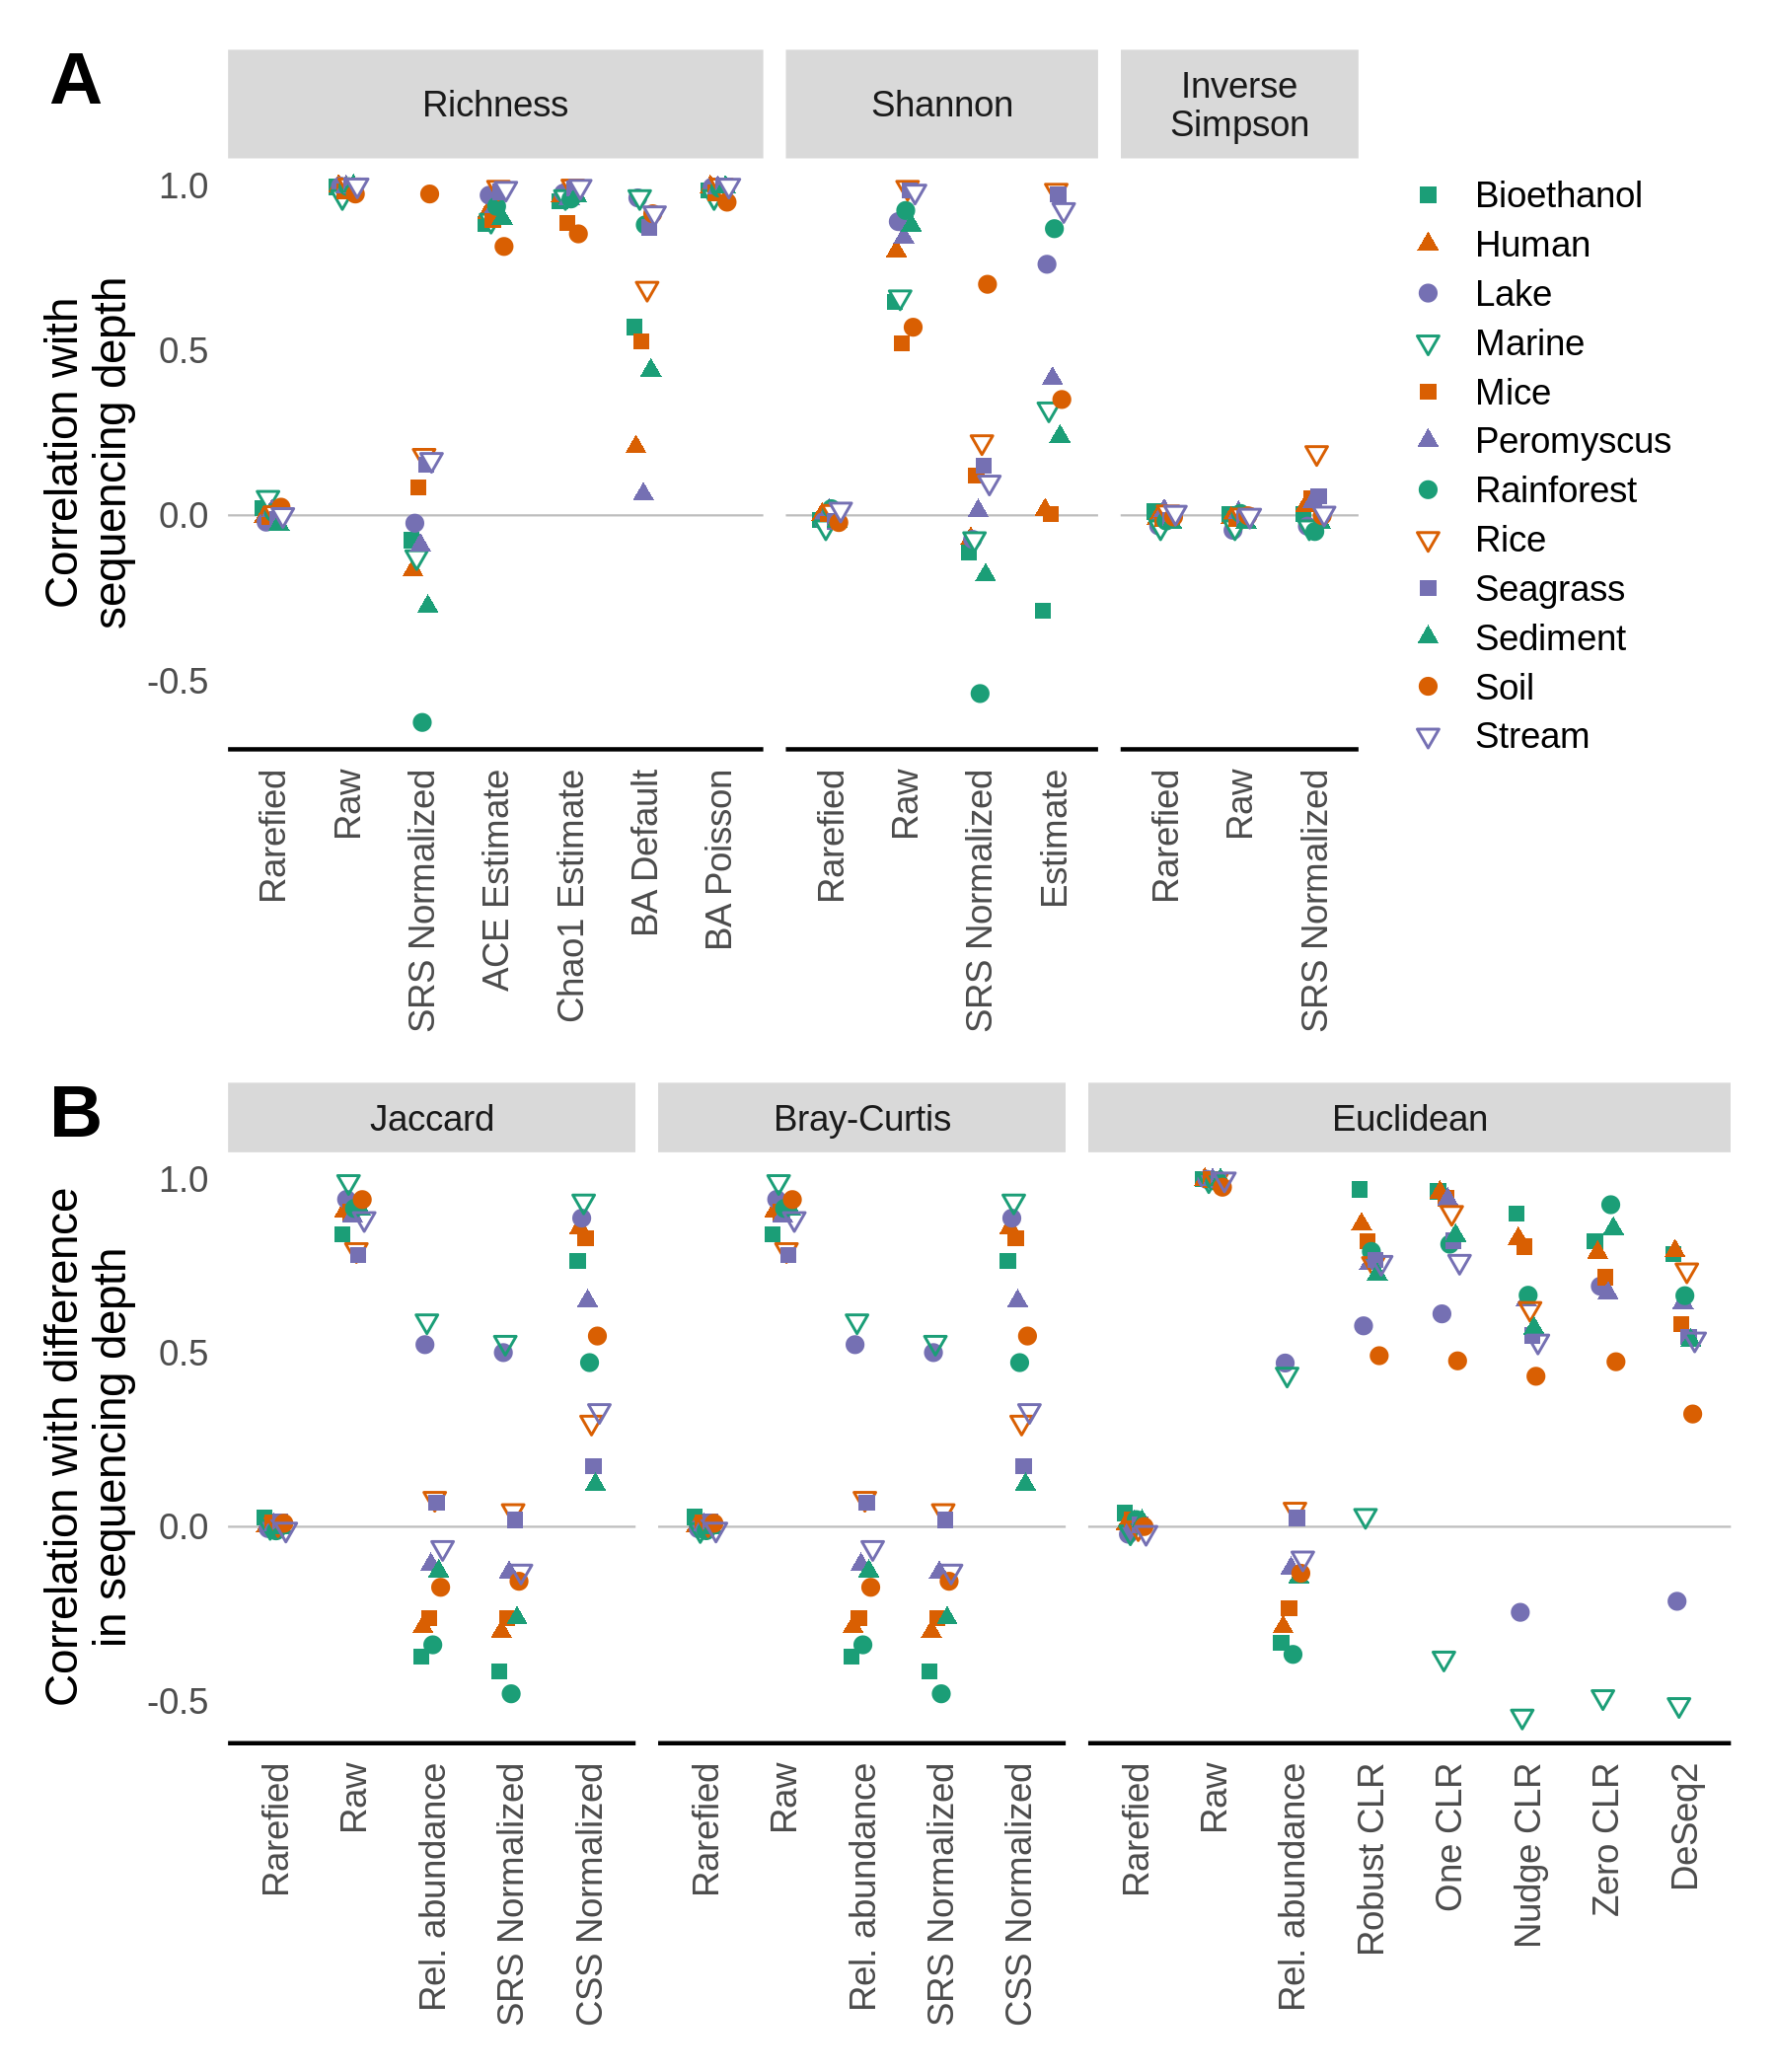
\includegraphics[height=17cm]{figure_1.png}

\textbf{Figure 1. Rarefaction eliminates the correlation between
sequencing depth and alpha diversity (A) and between differences in
sampling depth and beta (B) diversity metrics when using null community
models.} Examples of the relationship between different metrics and
methods for controlling for uneven sequencing effort are provided in
Figures S2 and S3 for alpha and beta diversity metrics, respectively.
Each point represents the mean of 100 random null community models; the
standard deviation was smaller than the size of the plotting symbol.

\newpage

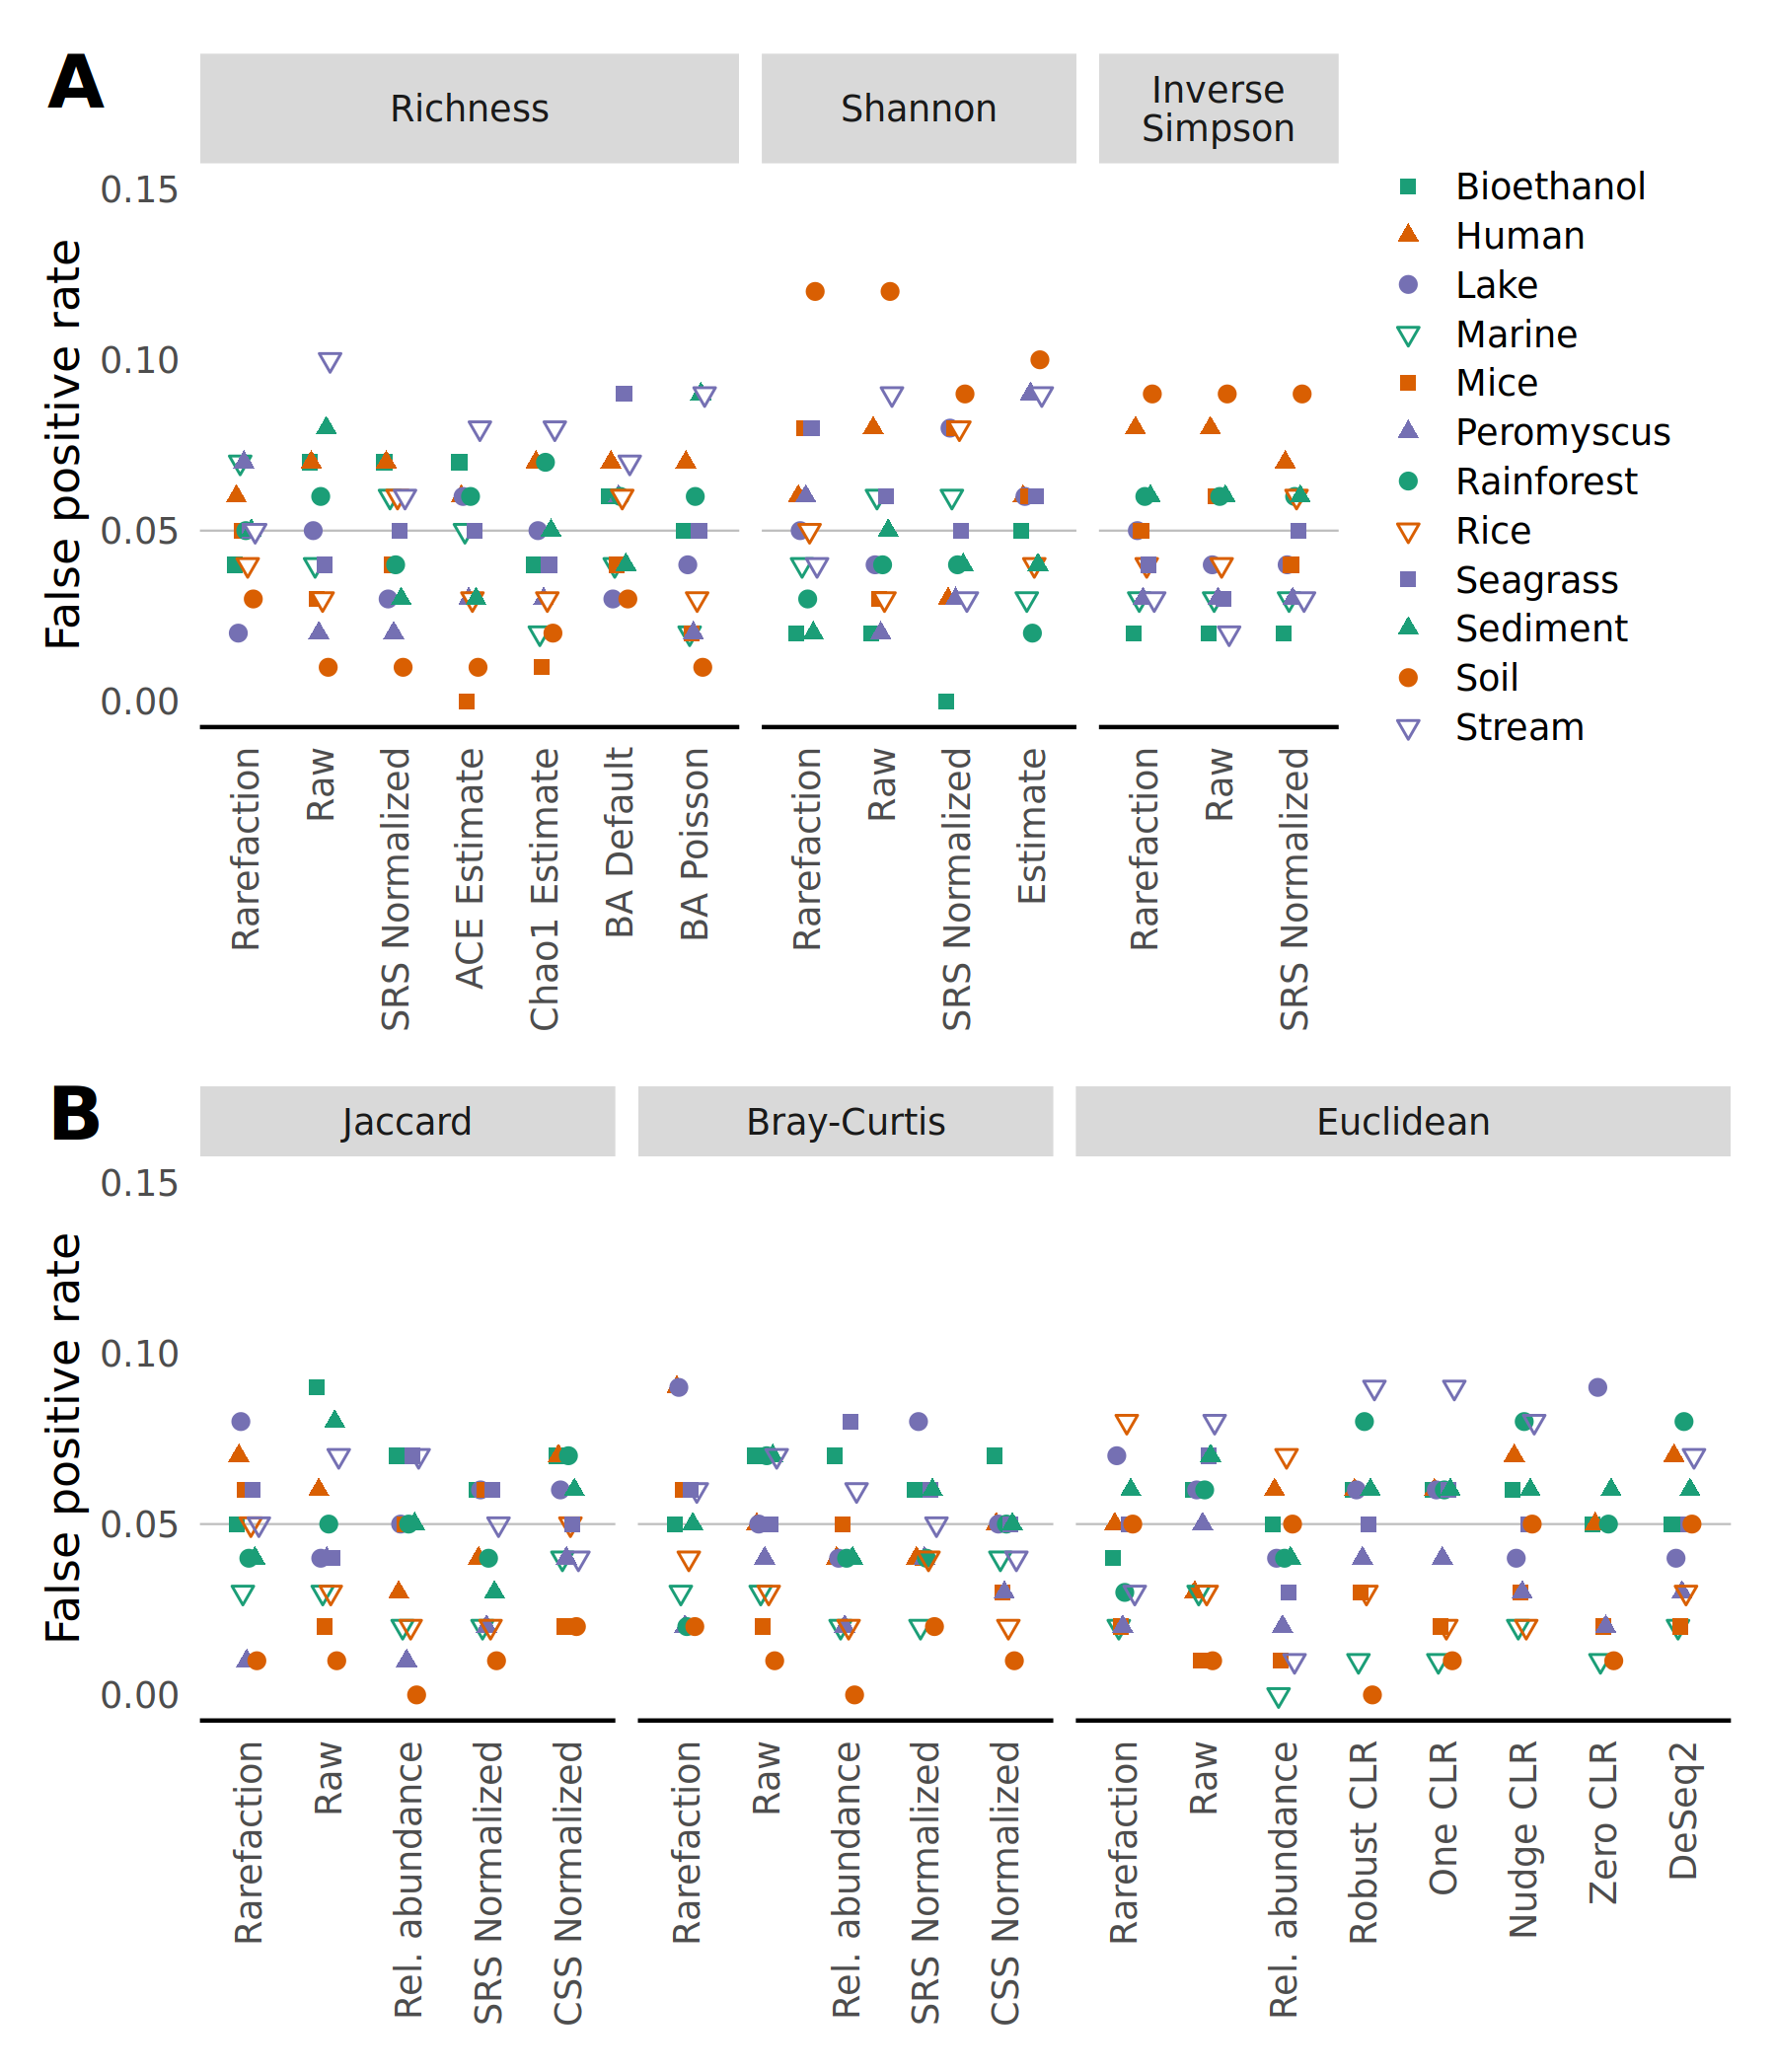
\includegraphics[height=17cm]{figure_2.png}

\textbf{Figure 2. The risk of falsely detecting a difference between
treatment groups drawn from a null model does not meaningfully vary from
5\%, regardless of approach for controlling for uneven sequencing
depth}. Samples were randomly assigned to different treatment groups. To
calculate the false detection rate, datasets were regenerated 100 times
and differences in alpha diversity were tested using a Wilcoxon test (A)
and differences in beta diversity were tested using PERMANOVA (B) at a
5\% threshold. The false positive rate was the number of times a dataset
yeilded a significant result.

\newpage

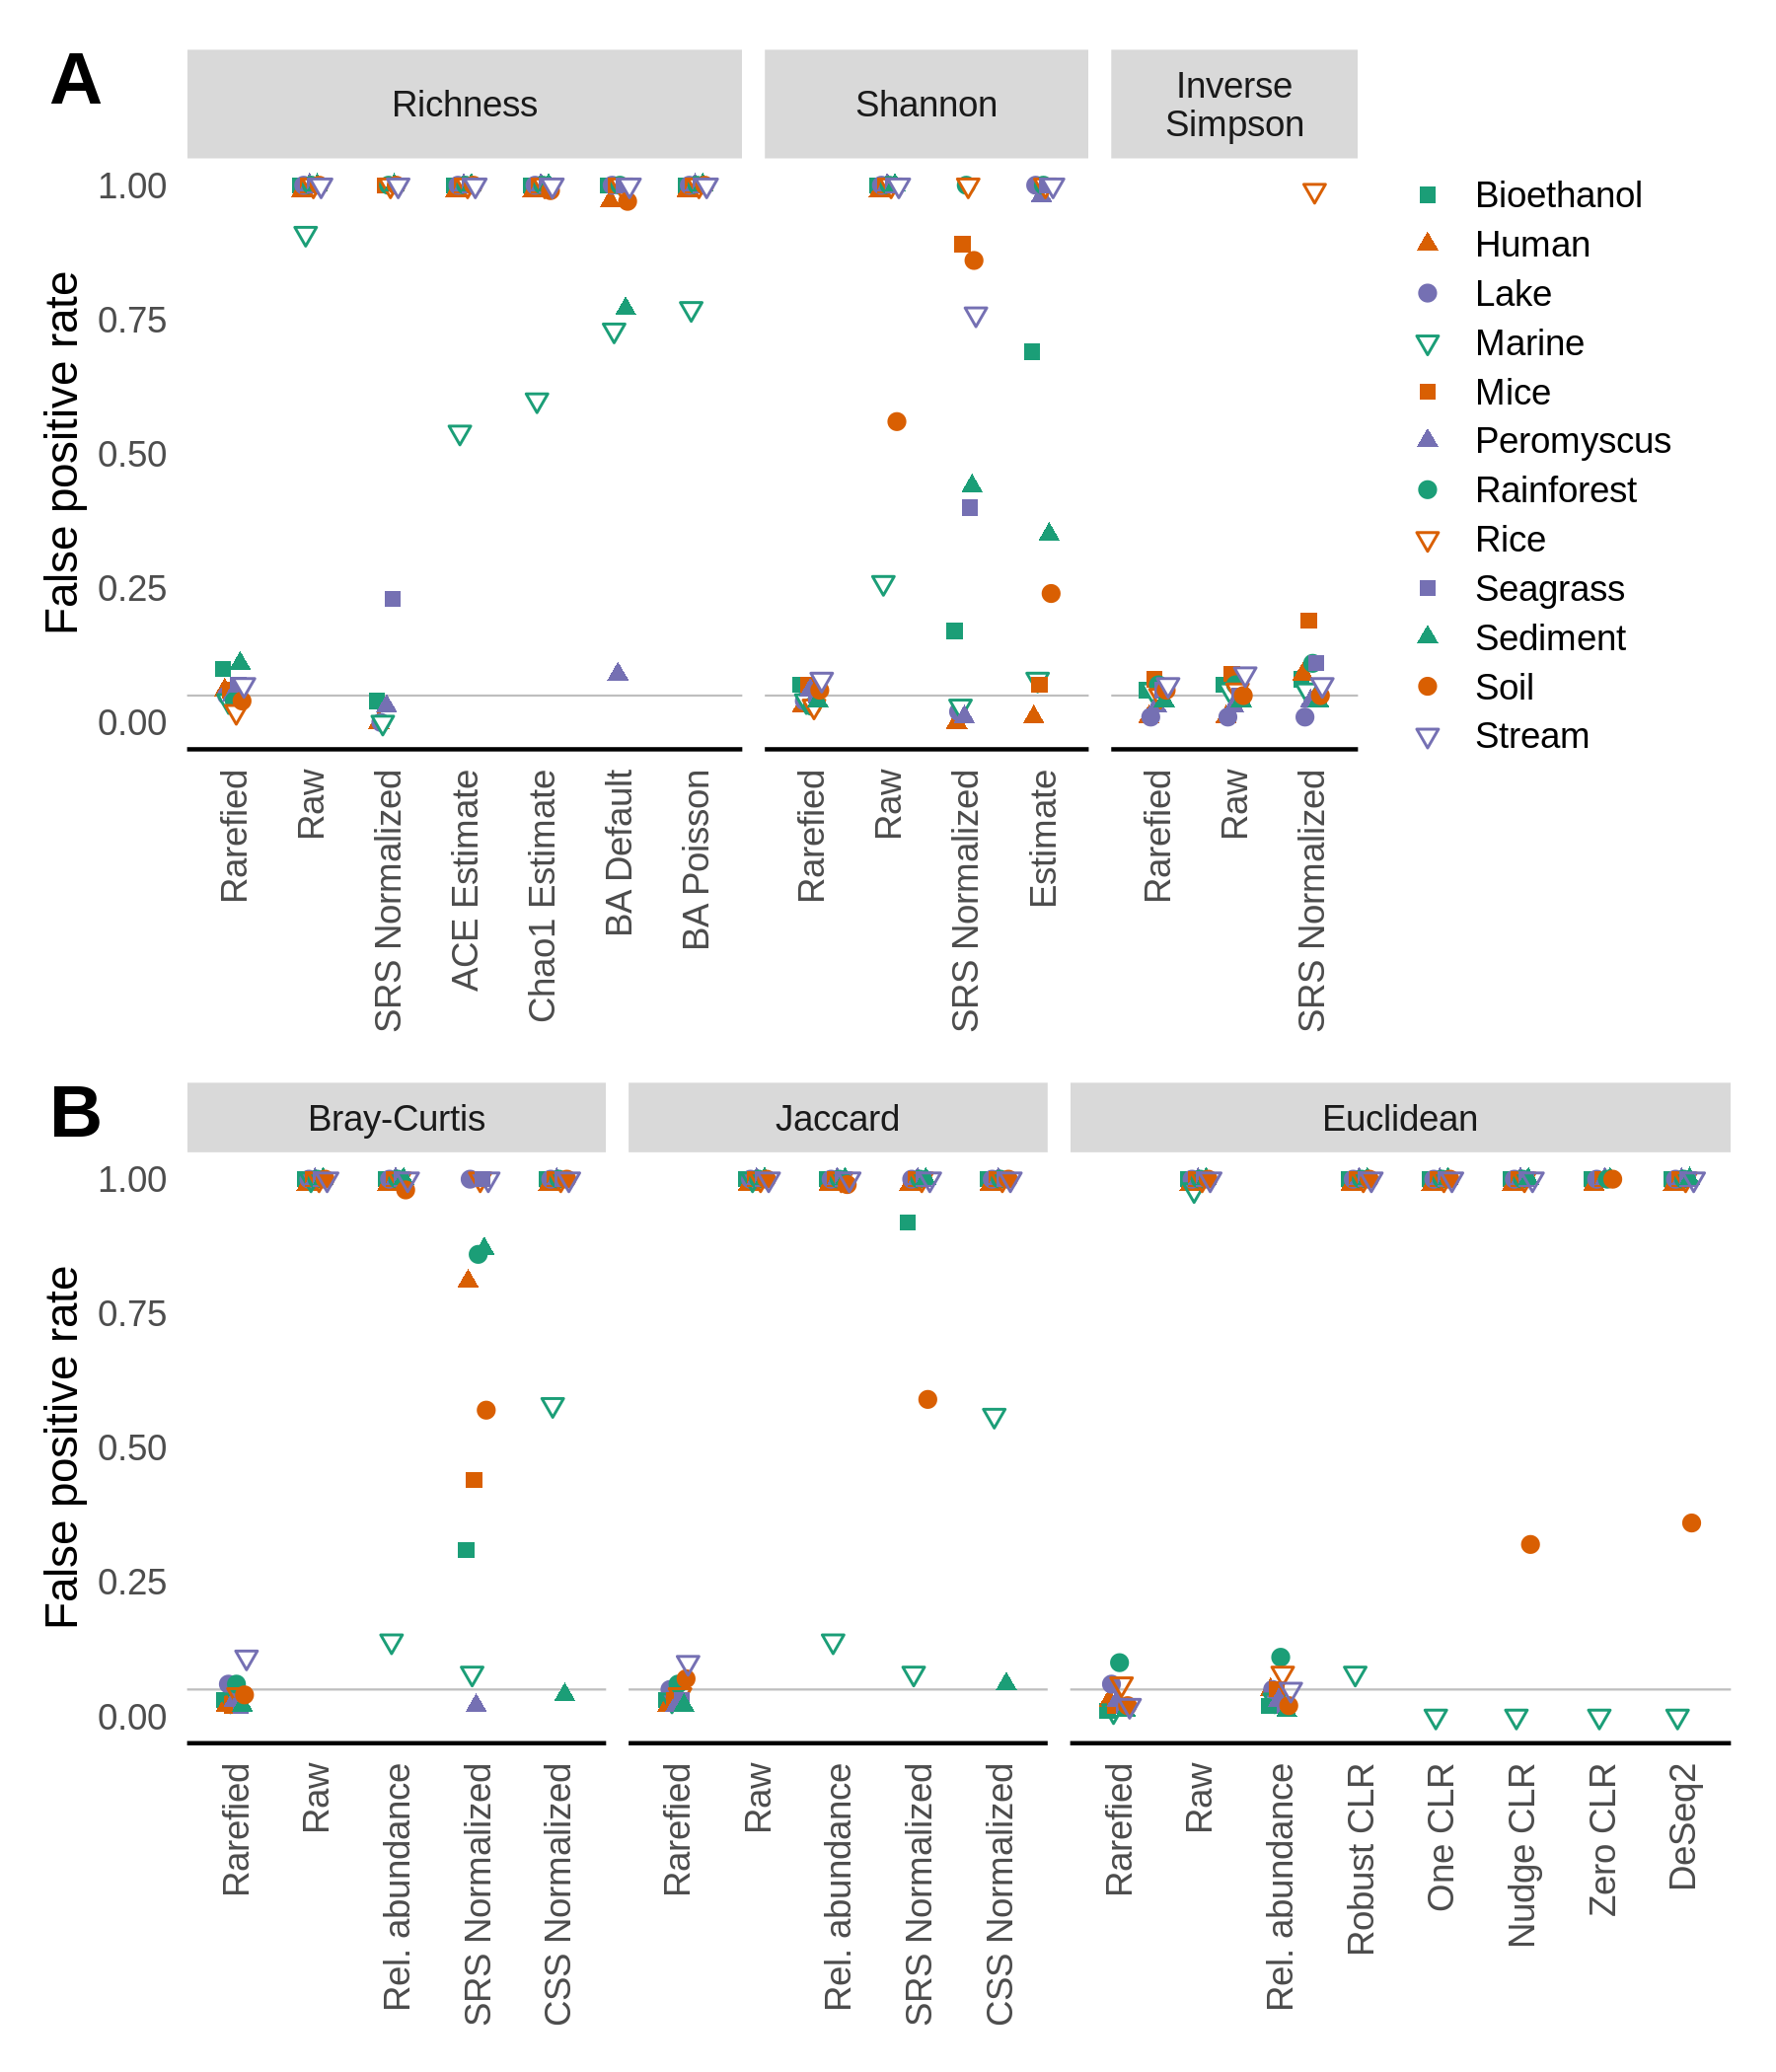
\includegraphics[height=17cm]{figure_3.png}

\textbf{Figure 3.The risk of falsely detecting a difference between
treatment groups drawn from a null model does not meaningfully vary from
5\% when data are rarefied when sequencing depth is confounded with
treatement group}. Samples were assigned to different treatment groups
based on whether they were above the median number of sequences for each
dataset. To calculate the false detection rate, datasets were
regenerated 100 times and differences in alpha diversity were tested
using a Wilcoxon test (A) and differences in beta diversity were tested
using PERMANOVA (B) at a 5\% threshold. The false positive rate was the
number of times a dataset yeilded a significant result.

\newpage

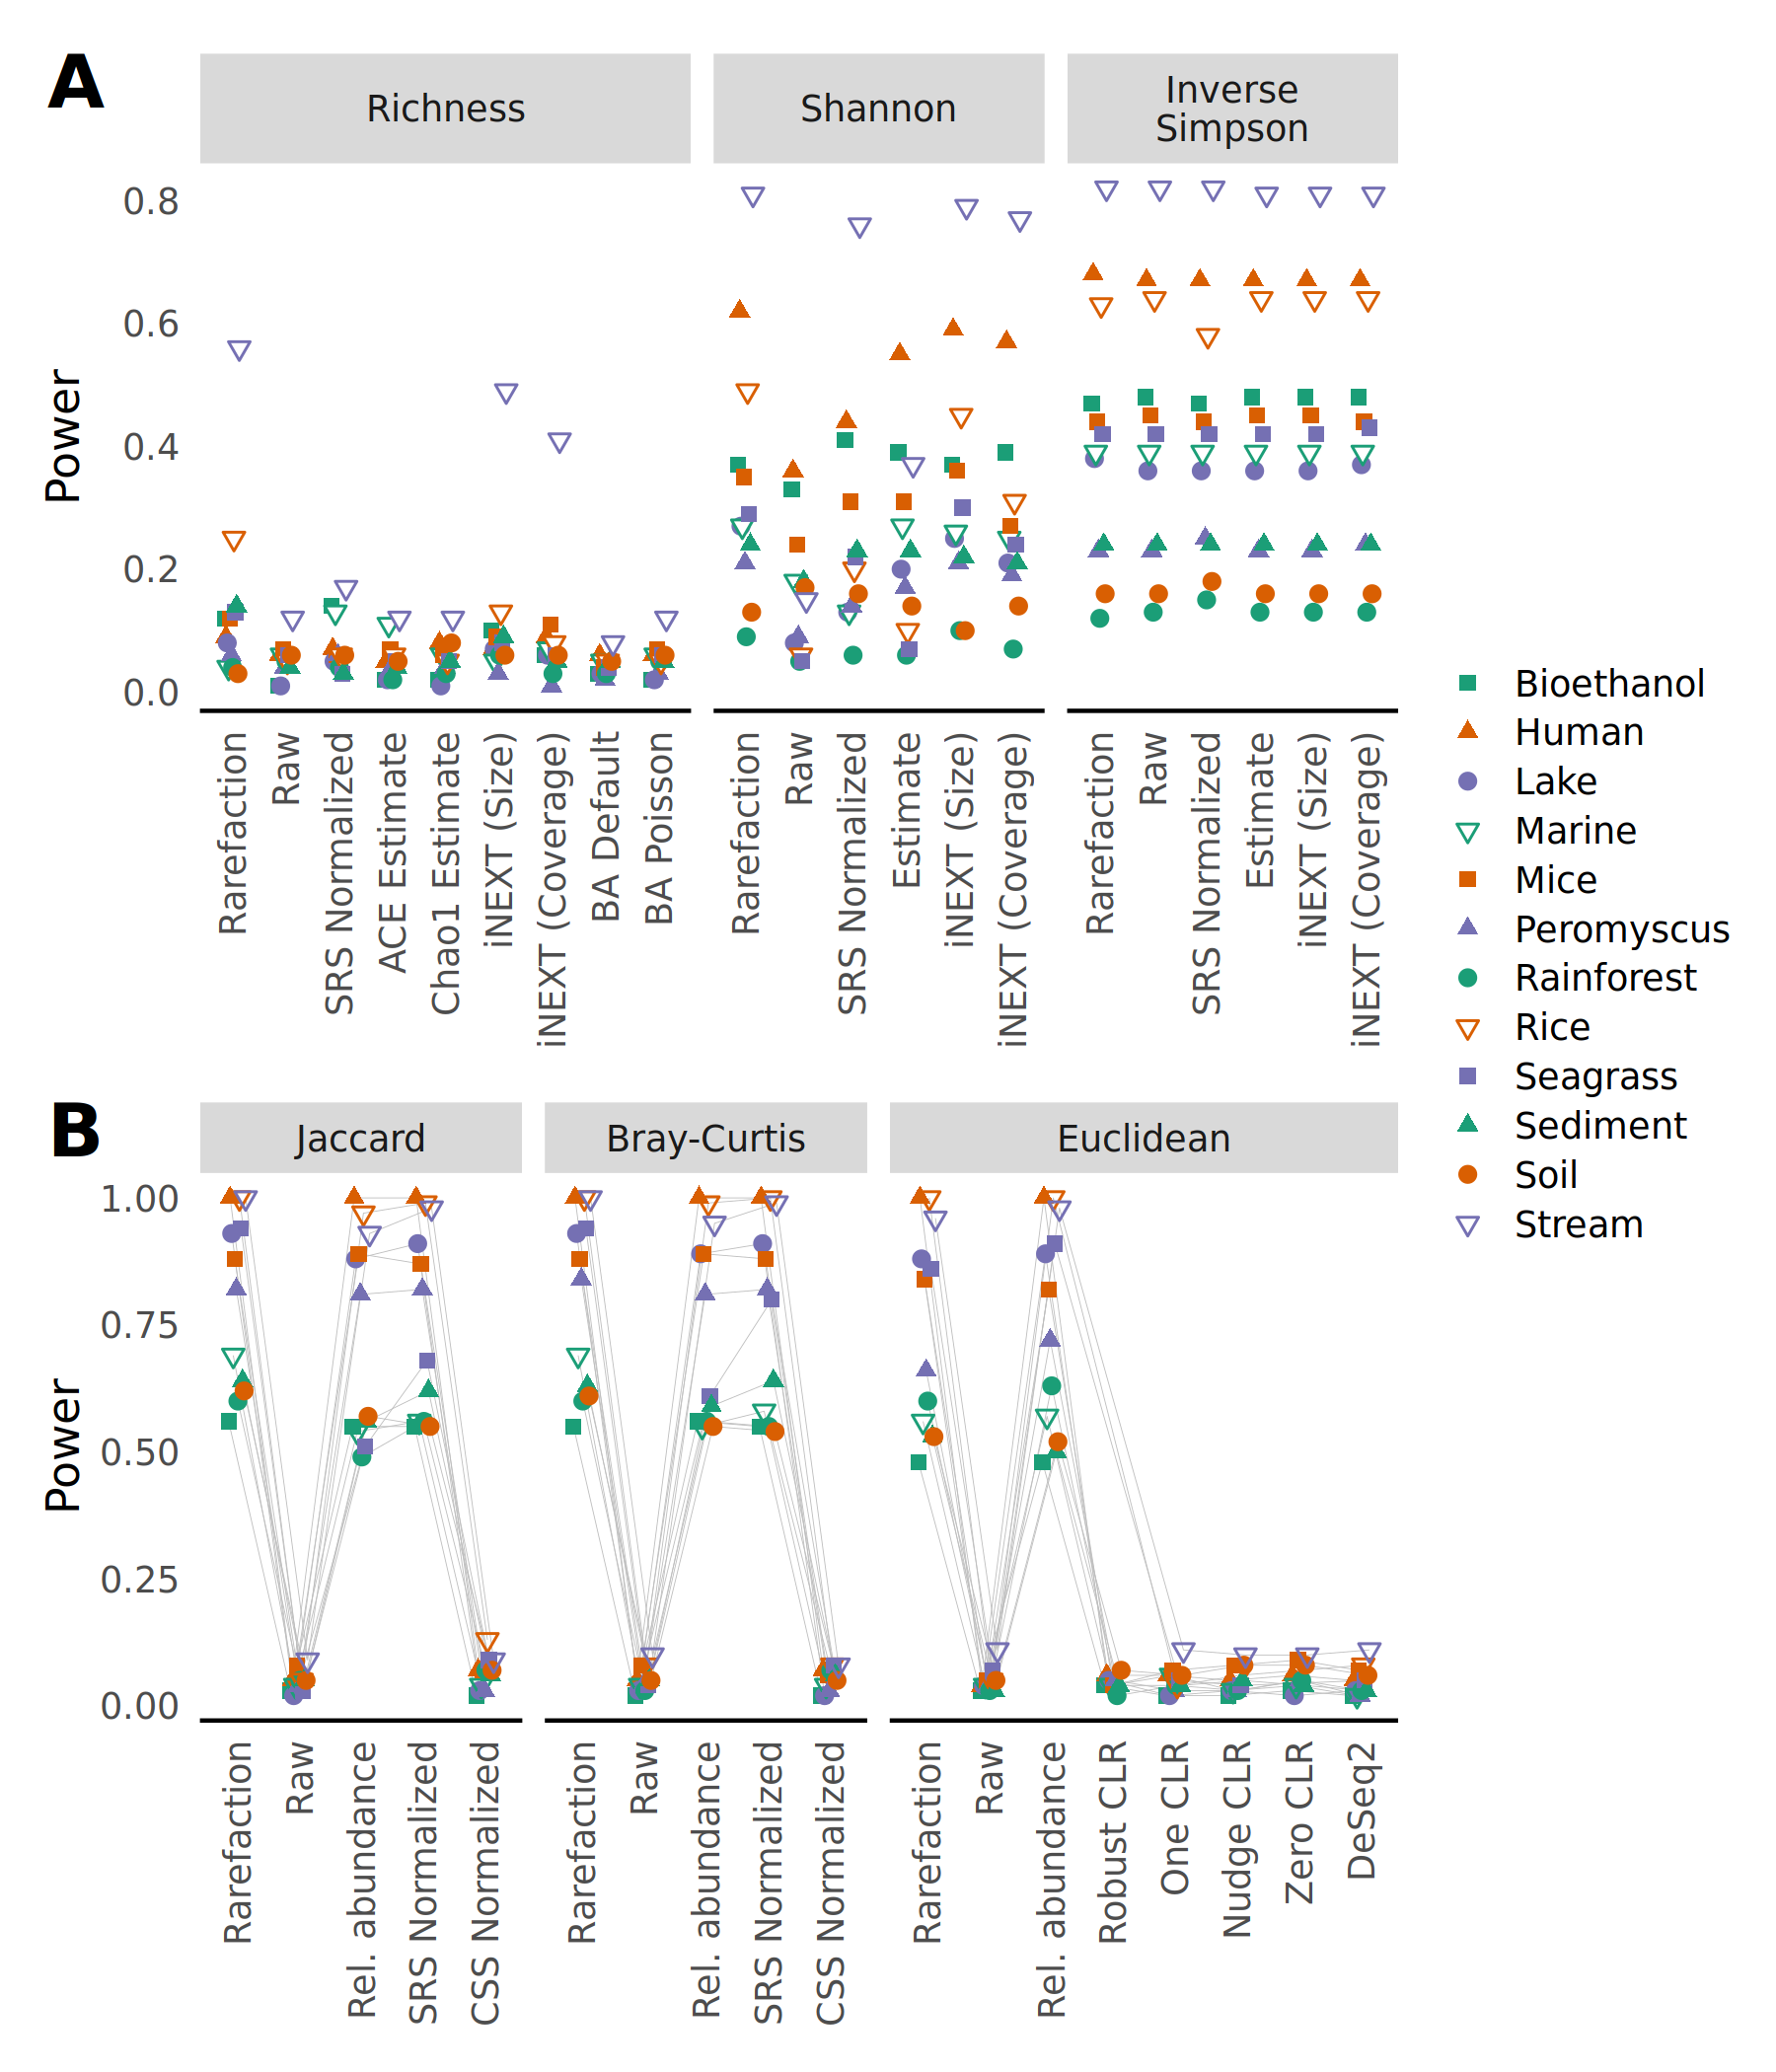
\includegraphics[height=17cm]{figure_4.png}

\textbf{Figure 4. The ability to detect true differences in treatment
groups for alpha (A) and beta (B) diversity metrics is greatest when
communities differing in the relative abundance of their OTUs are
rarefied.} For each dataset samples were randomly assigned to one of two
community distributions where the abundance of OTUs differed. To
calculate the power for each datasets, datasets were regenerated 100
times and differences in alpha diversity were tested using a Wilcoxon
test (A) and differences in beta diversity were tested using PERMANOVA
(B) at a 5\% threshold. The power was the number of times a dataset
yielded a significant result.

\newpage

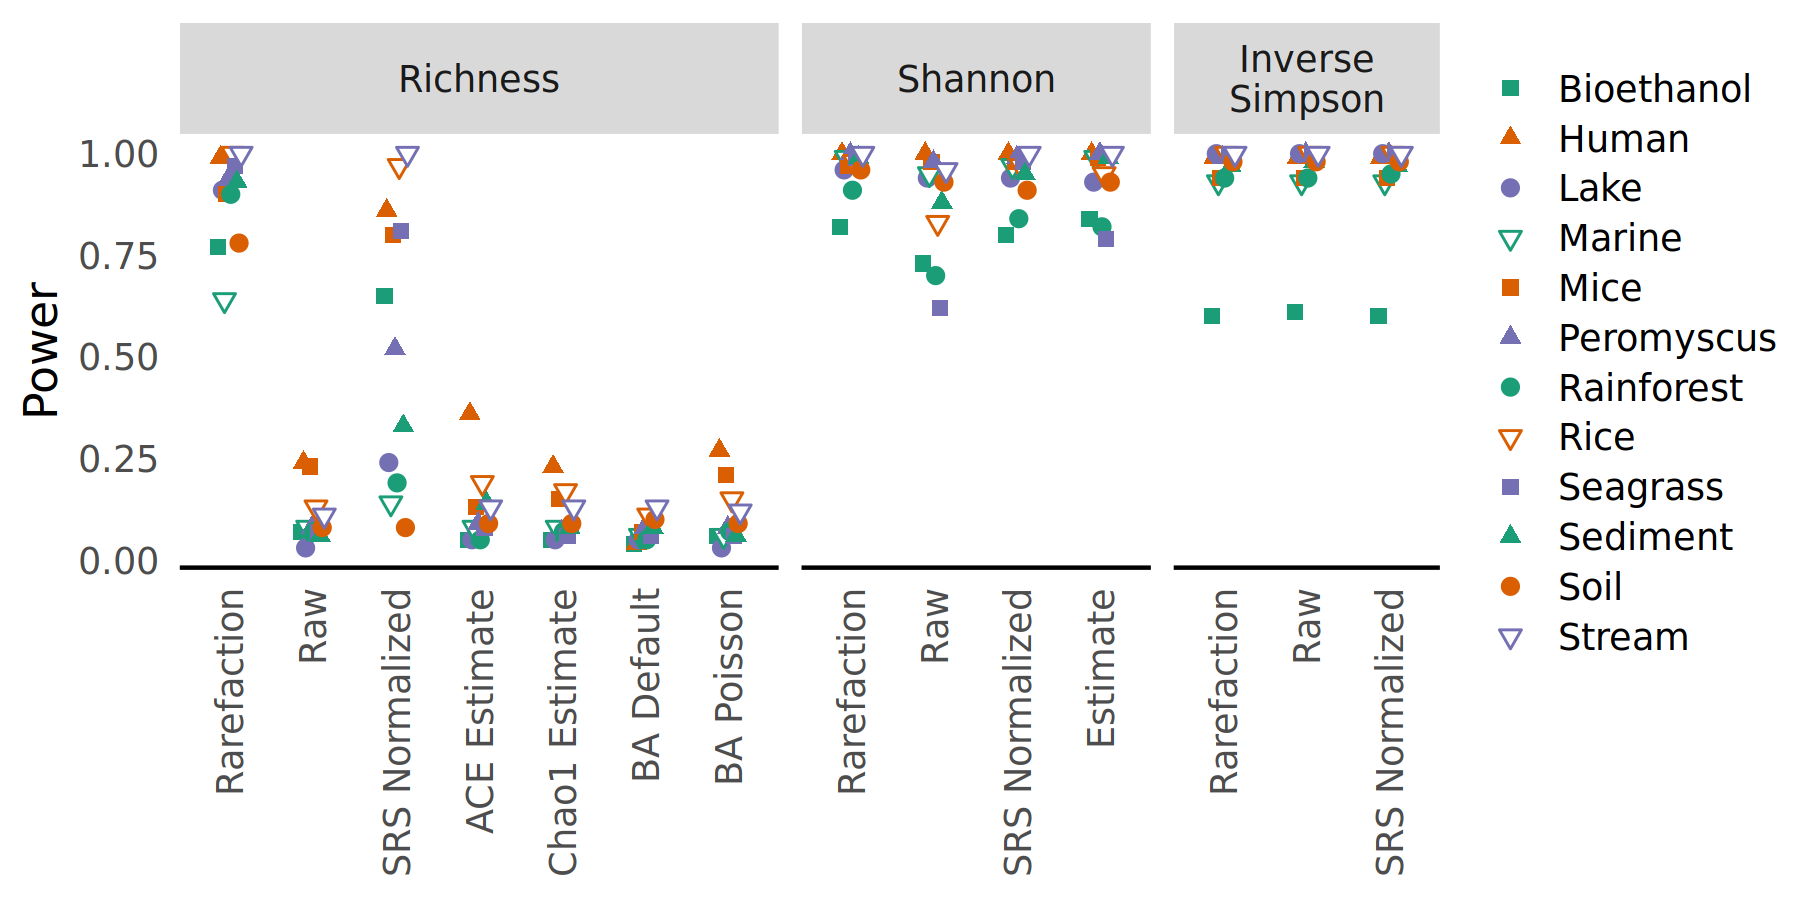
\includegraphics{figure_5.png}

\textbf{Figure 5. The ability to detect true differences in treatment
groups for alpha diversity metrics is greatest when communities
differing in richness are rarefied.} For each dataset samples were
randomly assigned to one of two community distributions where one
distribution contained a subset of OTUs found in the other. To calculate
the power for each dataset, datasets were regenerated 100 times and
differences in alpha diversity were tested using a Wilcoxon test (A) and
differences in beta diversity were tested using PERMANOVA (B) at a 5\%
threshold. The power was the number of times a dataset yielded a
significant result.

\newpage

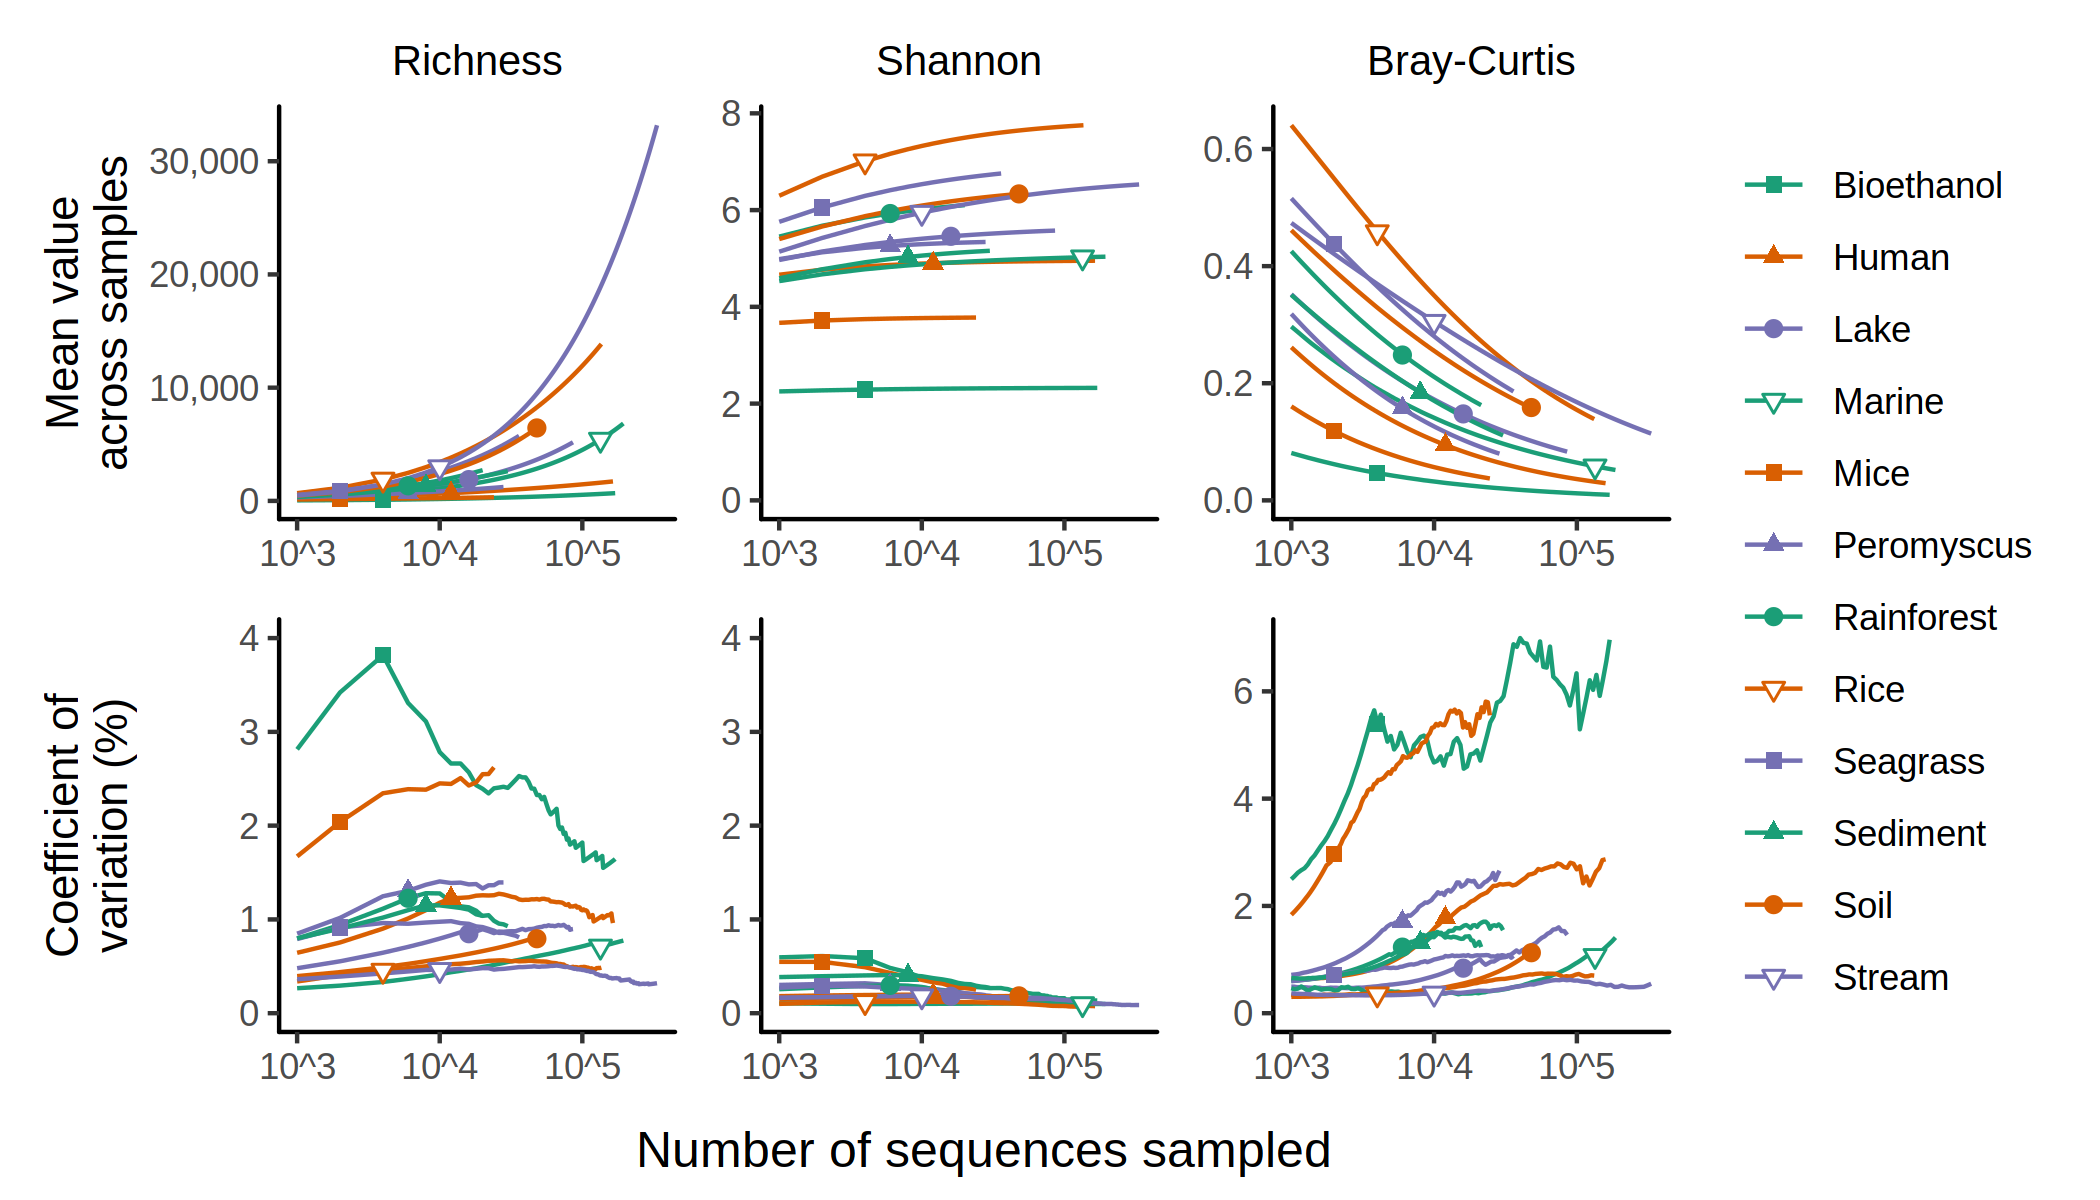
\includegraphics{figure_6.png}

\textbf{Figure 6. The mean and coefficient of variation for rarefied
richness, shannon diversity, and Bray-Curtis dissimilarity vary with
sequencing depth.} For each dataset, a null community distribution was
created and samples were created to have the same sequencing depth as
they did originally. The placement of the plotting symbol indicates the
size of the smallest sample. Results are only shown for sequencing
depths where a dataset had 5 or more samples.

\newpage

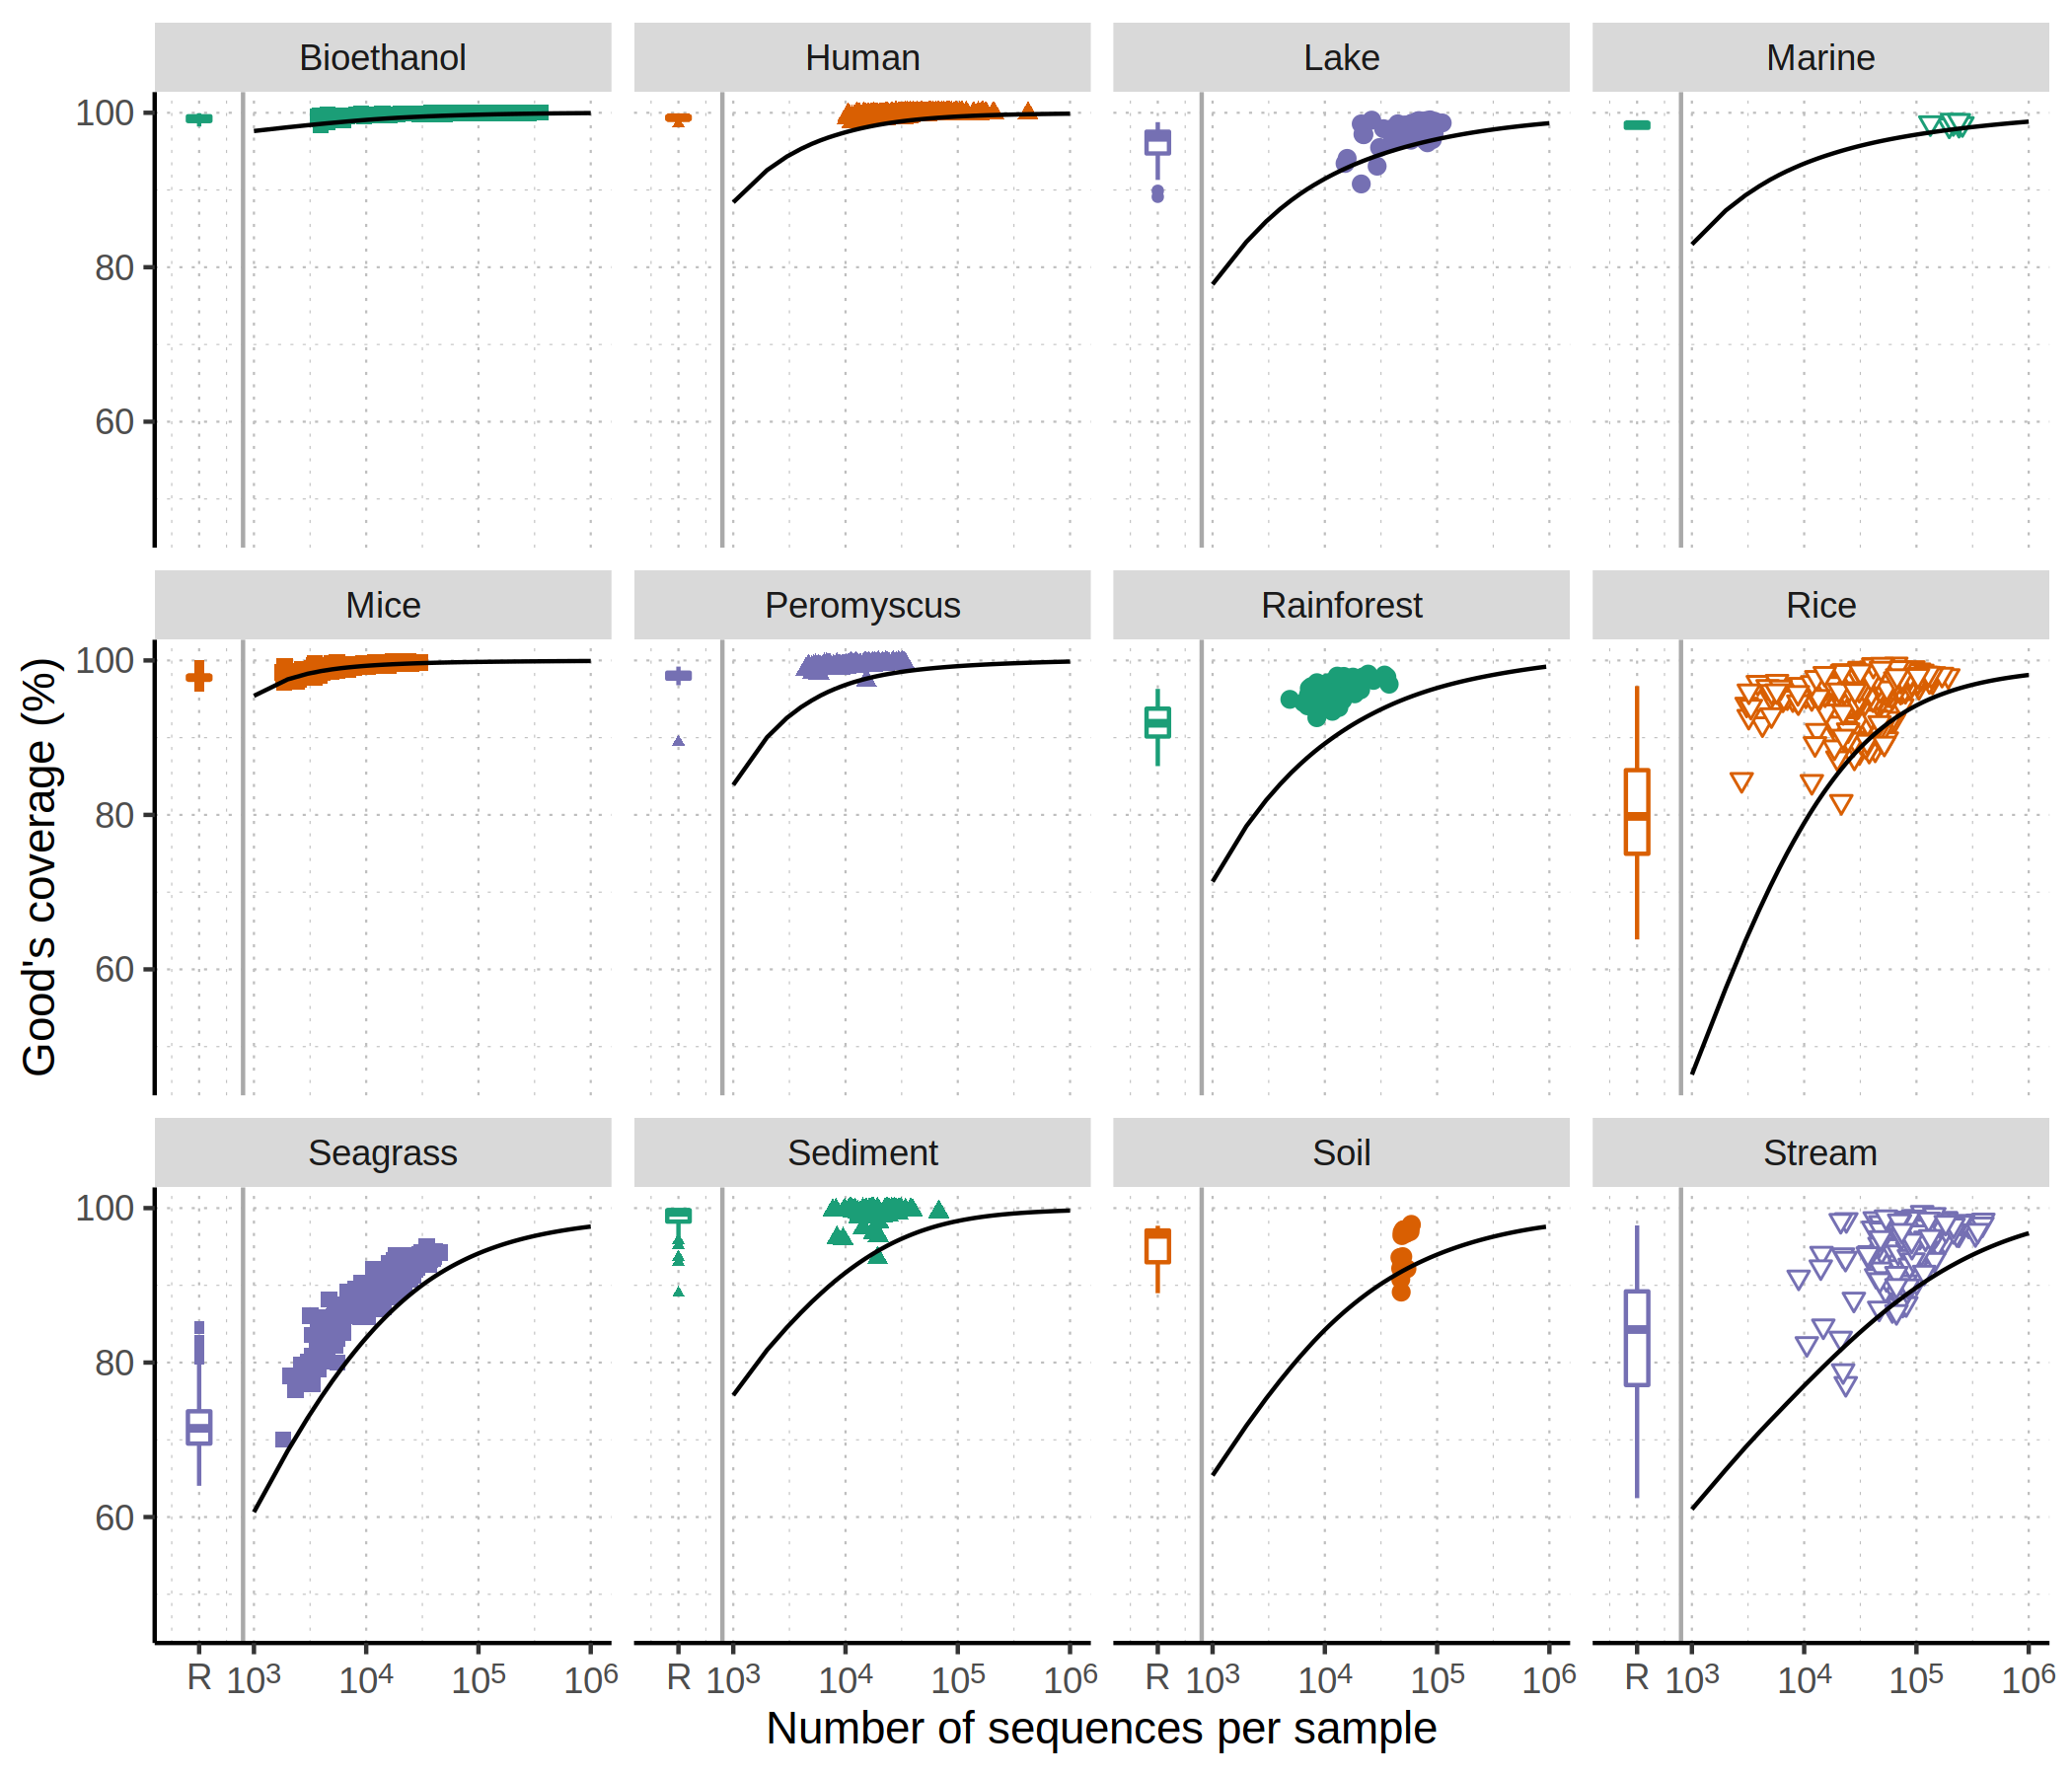
\includegraphics{figure_7.png}

\textbf{Figure 7. Most datasets are sequenced to a level that provides a
high level of coverage.} Each plotting symbol represents the observed
Good's coverage for a different sample in each dataset. The smoothed
line indicates the simulated coverage for varying levels of sampling
effort when a null community is generated from the observed data. The
box and whisker plot indicates the range of coverage values when the
observed commmunity data were rarefied to the size of the least
sequenced sample.

\newpage

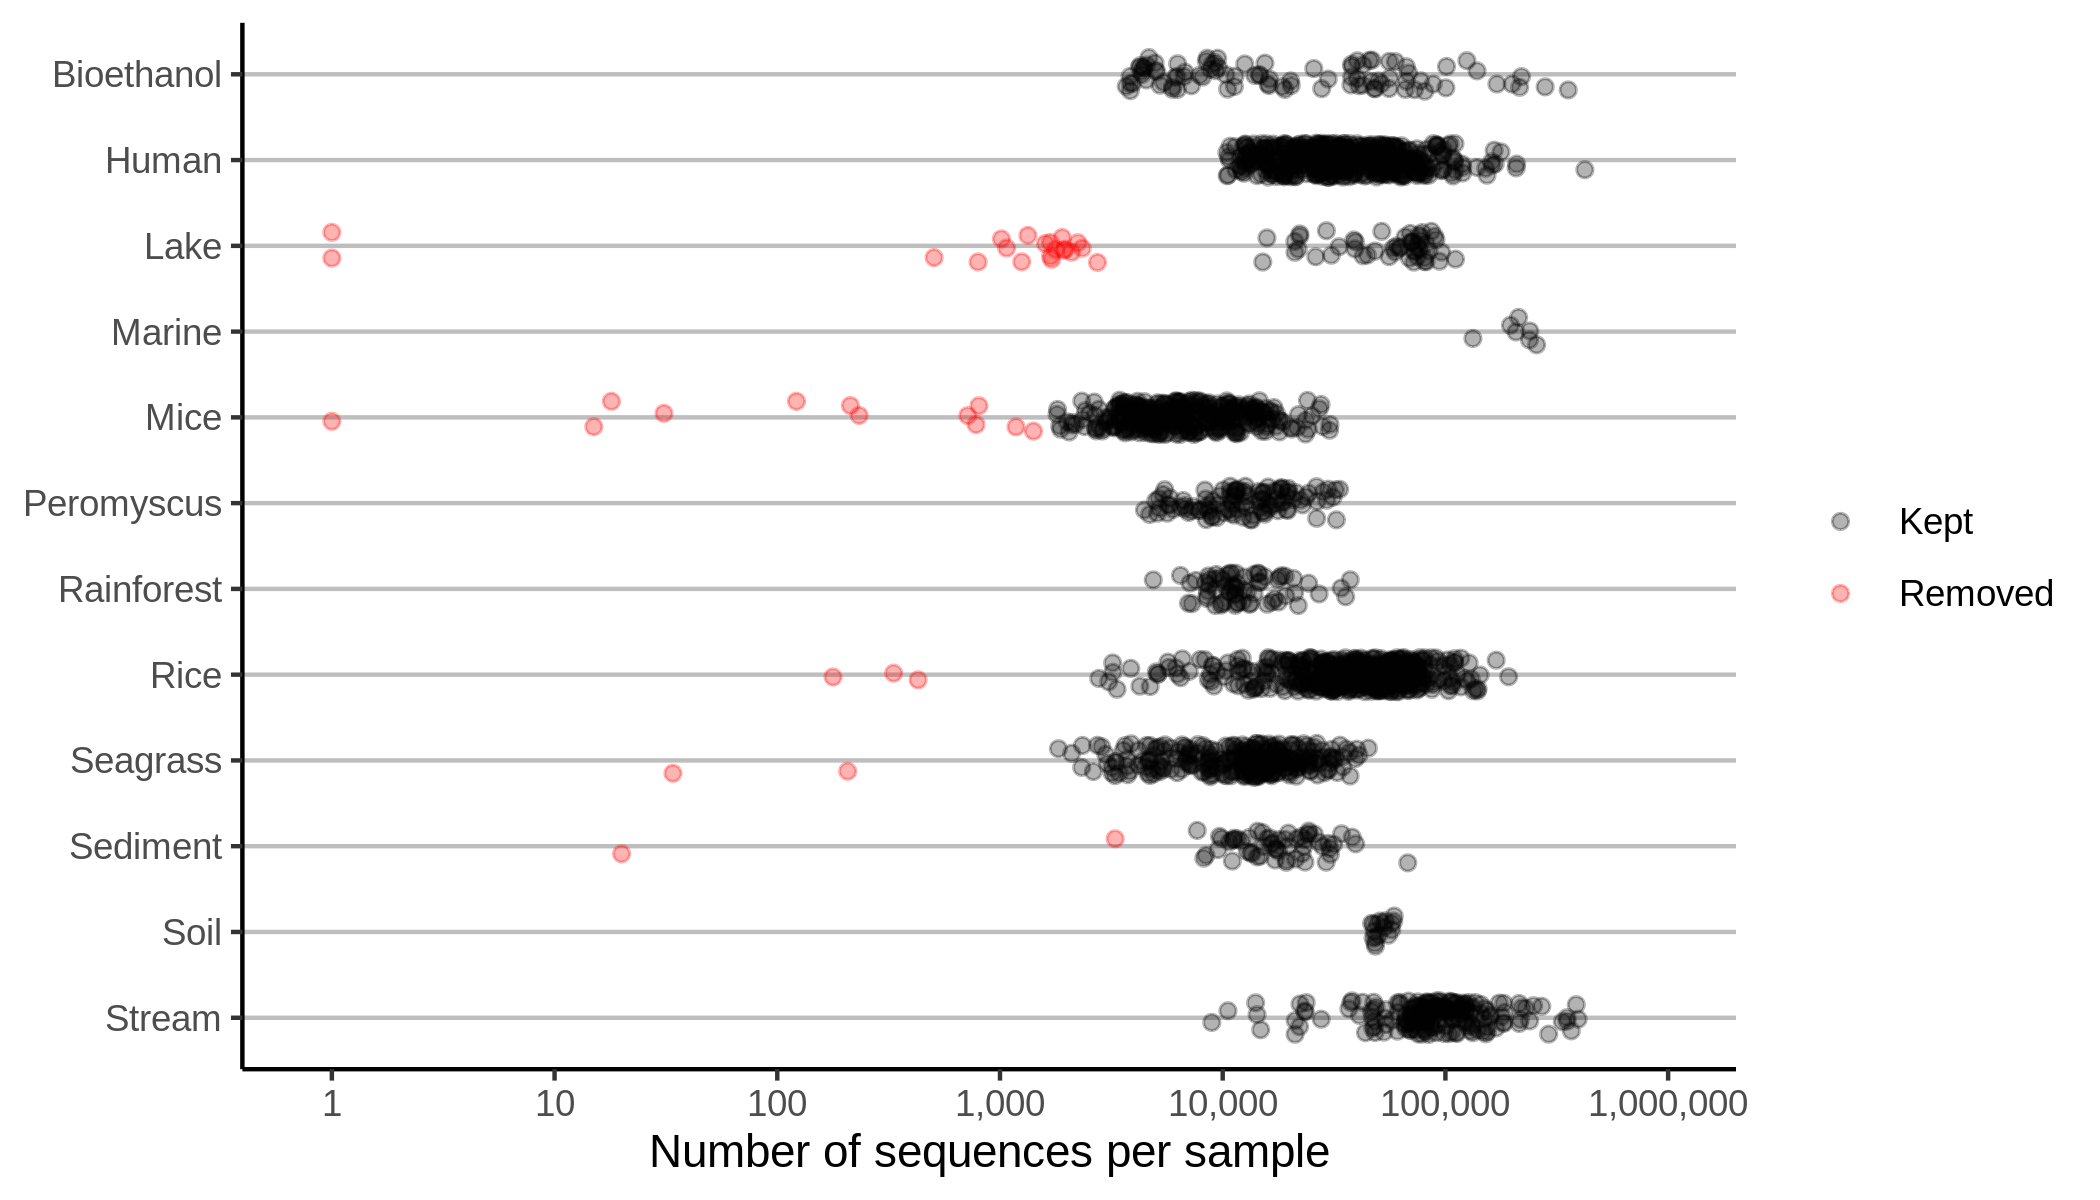
\includegraphics{figure_s1.png}

\textbf{Figure S1. The number of sequences observed in each sample for
each dataset included in this analysis generally varied by 10 to
100-fold.} The threshold for specifying the number of sequences per
sample varied by dataset and was determined based on identifying natural
breaks in the data.

\newpage

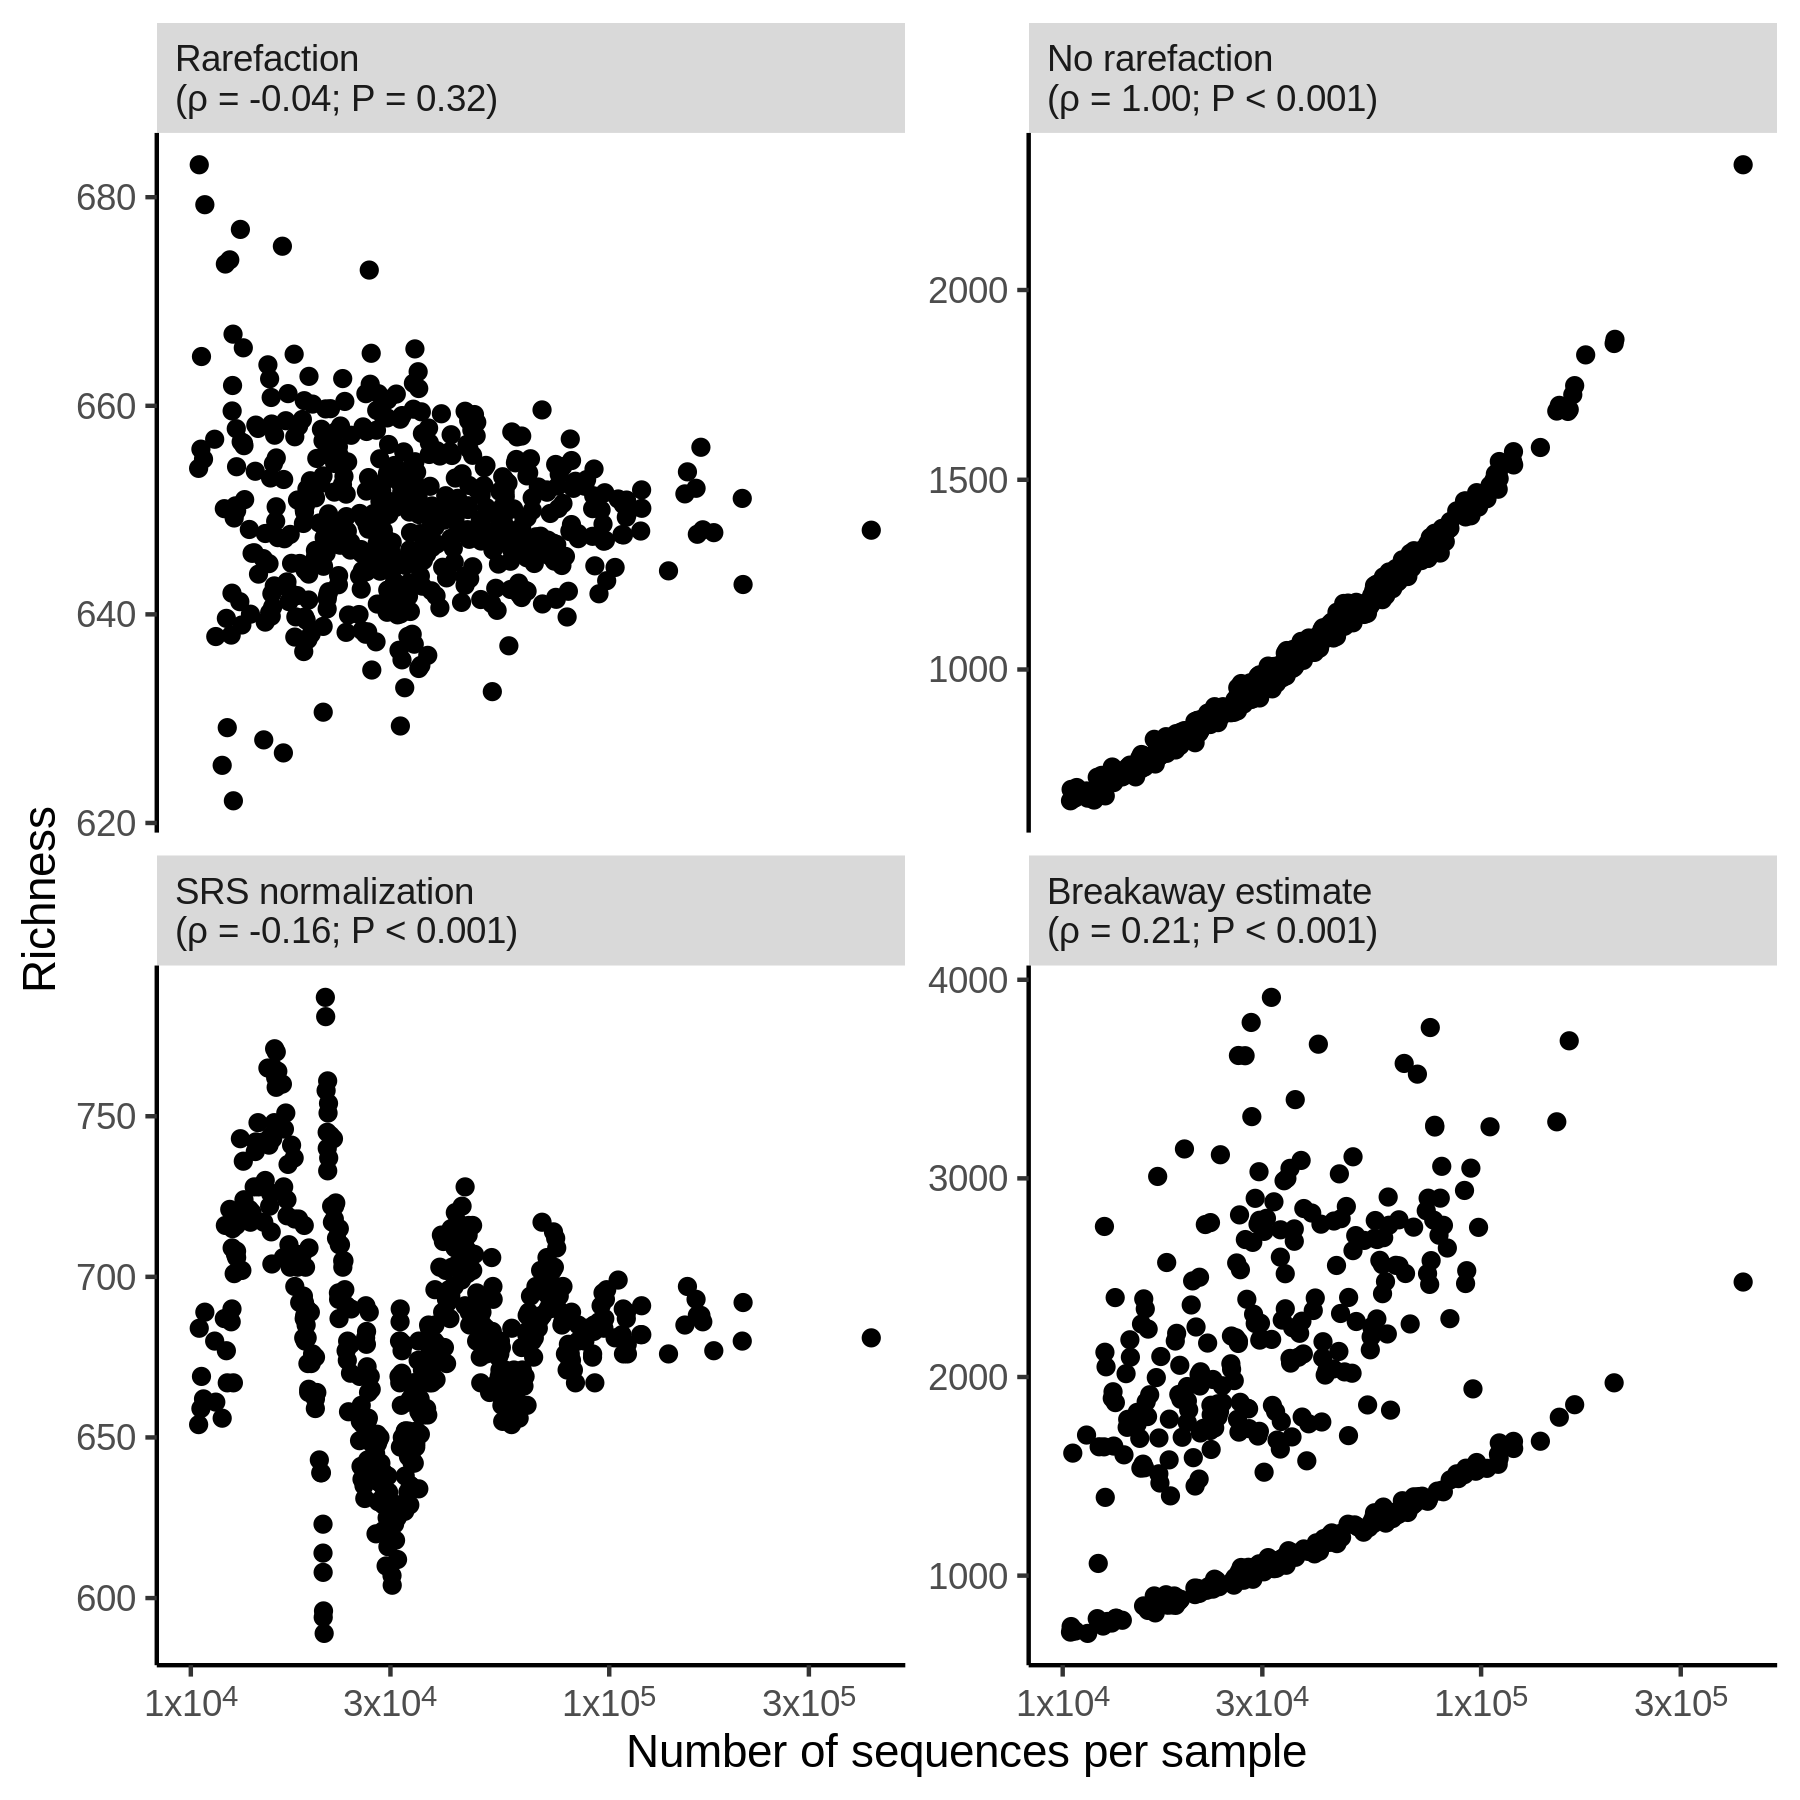
\includegraphics{figure_s2.png}

\textbf{Figure S2. Examples of the richness in each of the 490 samples
that were generated for one randomization of the null model using the
human dataset.} The x-axis indicates the number of sequences in each of
the samples prior to each method's appraoch of controlling for uneven
sampling effort. The Spearman correlation coefficient (\(\uprho\)) and
test of whether the coefficient was significantly different from zero
are indicated for each panel.

\newpage

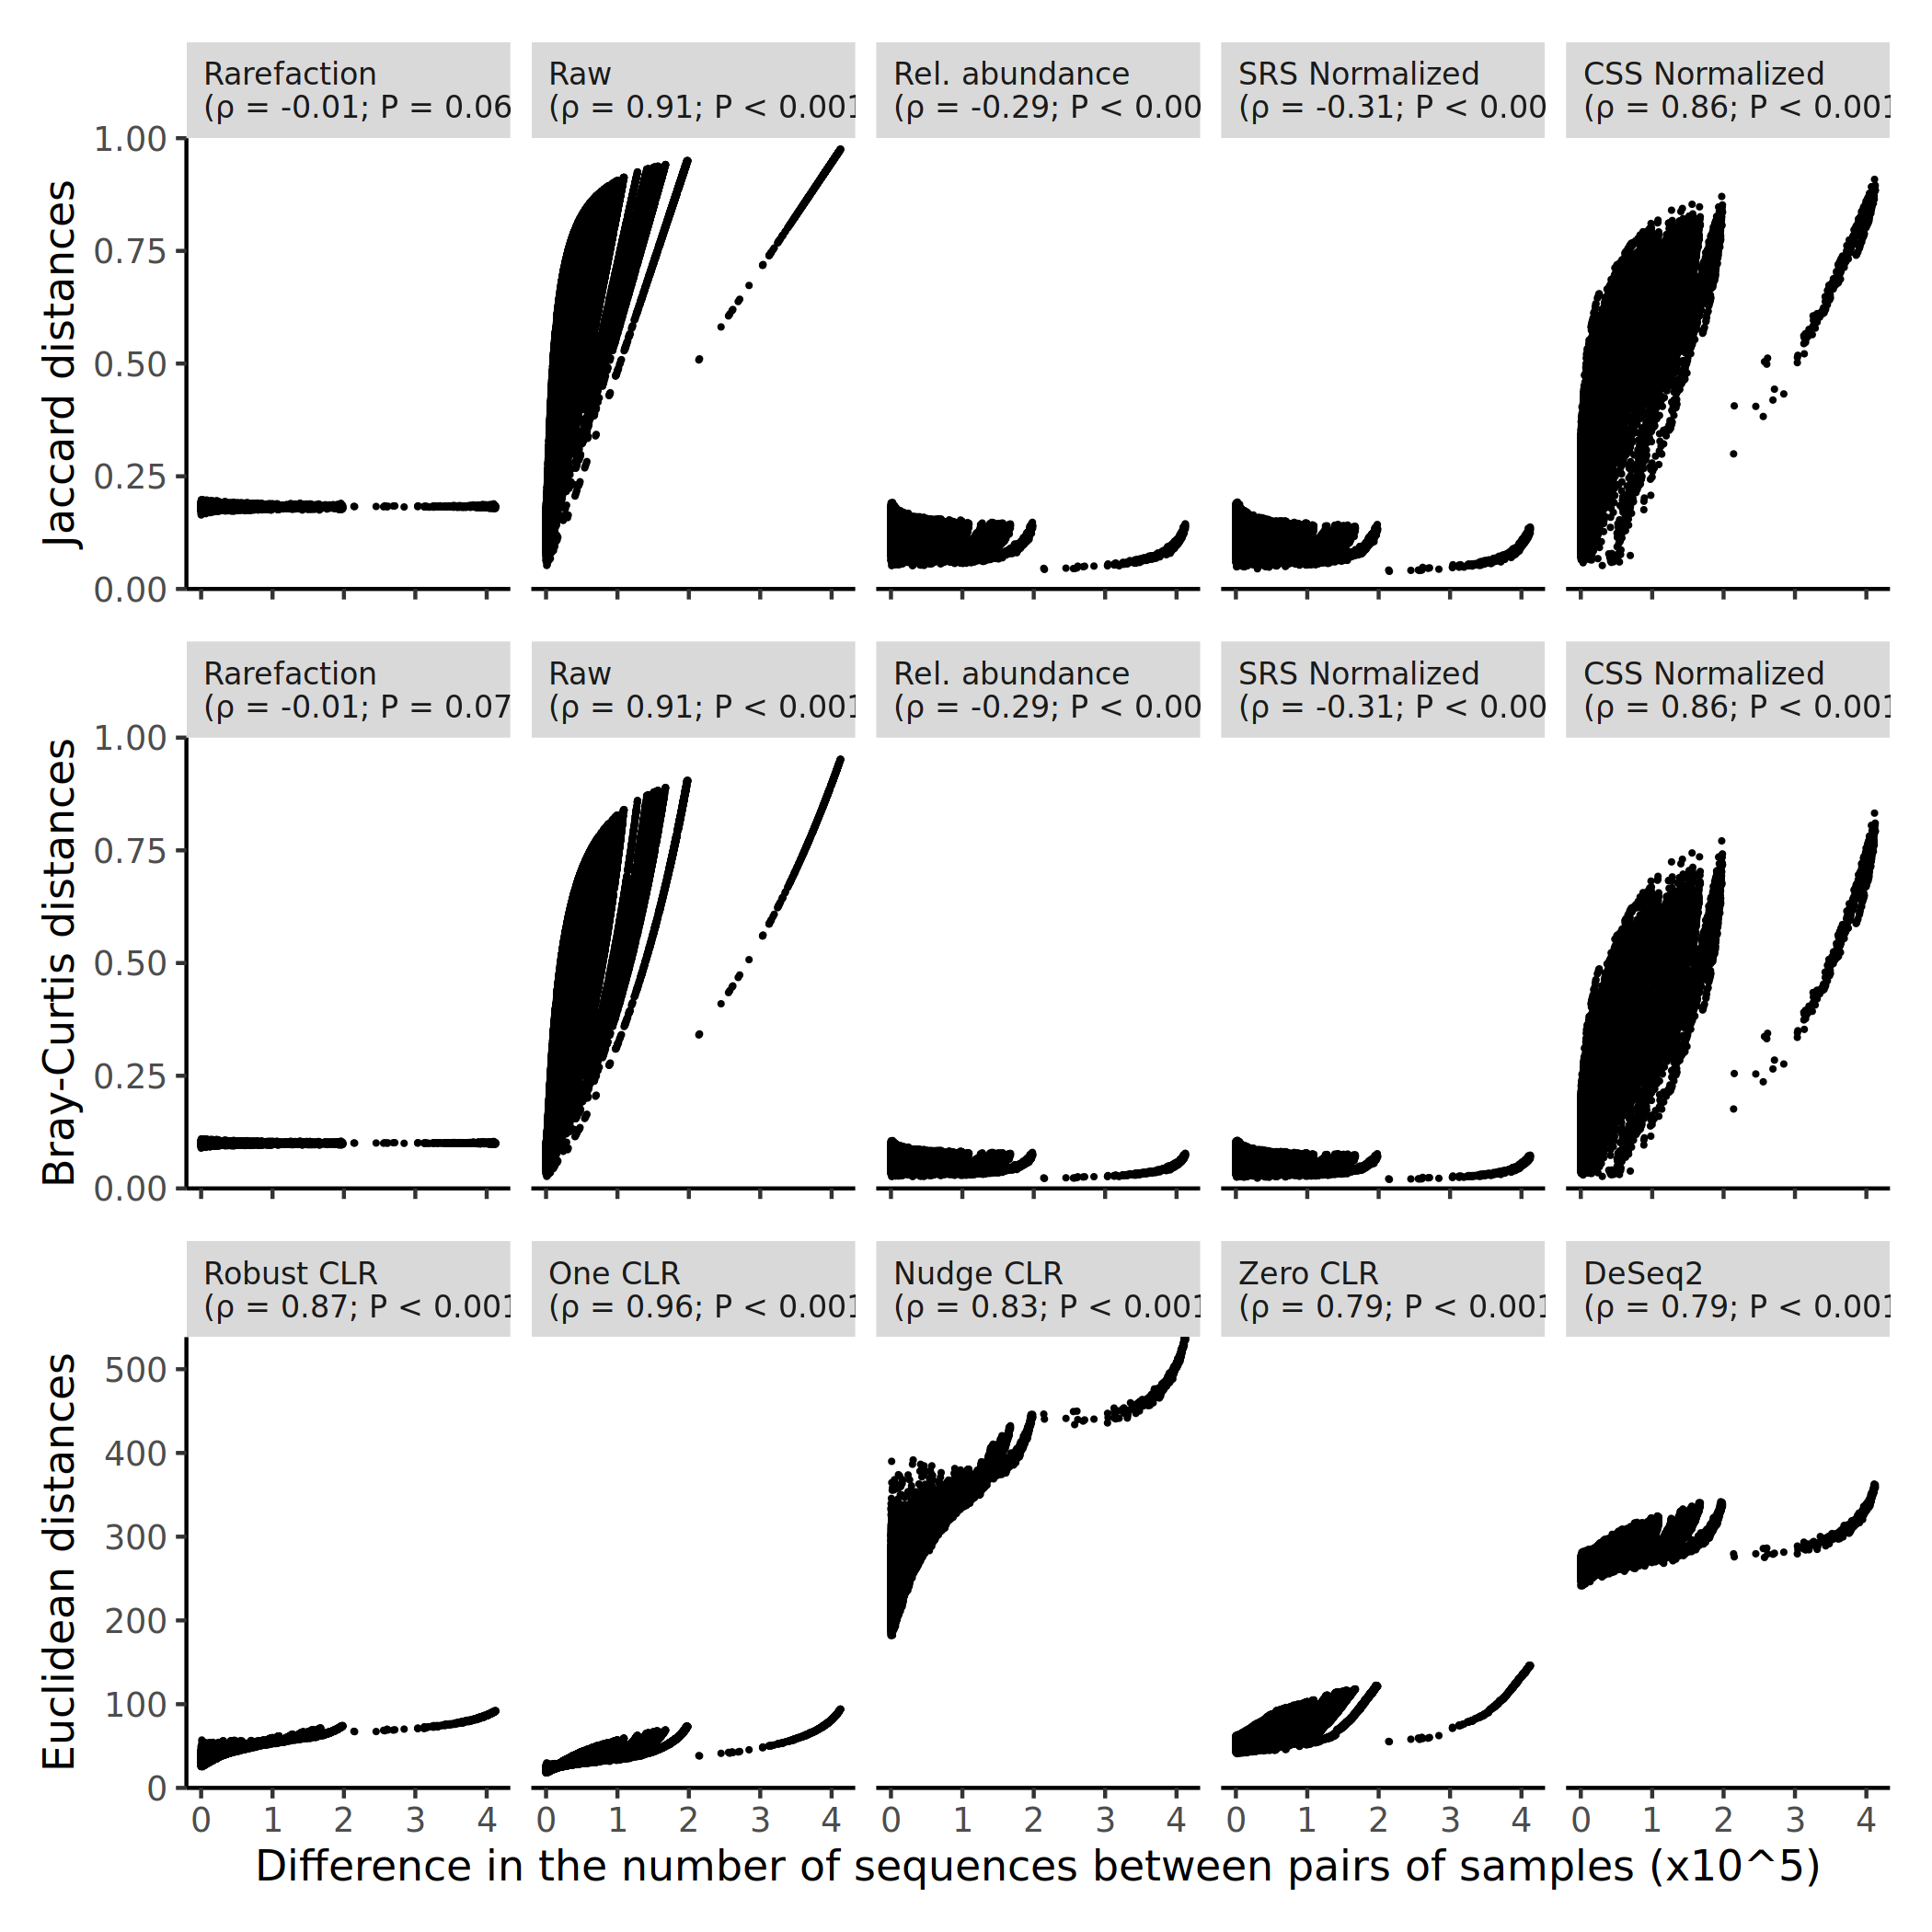
\includegraphics{figure_s3.png}

\textbf{Figure S3. Examples of differences in beta diversity in each of
the 490 samples that were generated for one randomization of the null
model using the human dataset.} The x-axis indicates the difference in
the number of sequences in each of the samples that went into
calcualting the pairwise distance prior to each method's appraoch of
controlling for uneven sampling effort. The Spearman correlation
coefficient (\(\uprho\)) and test of whether the coefficient was
significantly different from zero are indicated for each panel.

\end{document}
